\documentclass[12pt,a4paper]{article}
\usepackage{amsmath}

% Bibliografía %
\usepackage[backend=biber]{biblatex}
\addbibresource{referencias.bib} %Imports bibliography file
\usepackage[nottoc,numbib]{tocbibind}

\usepackage{vmargin}
\setpapersize{A4}
\setmargins{2.5cm}       % margen izquierdo
{1.5cm}                        % margen superior
{16.5cm}                      % anchura del texto
{23.42cm}                    % altura del texto
{10pt}                           % altura de los encabezados
{1cm}                           % espacio entre el texto y los encabezados
{0pt}                             % altura del pie de página
{2cm}                           % espacio entre el texto y el pie de página


\usepackage{amsfonts}
\usepackage{amssymb}
\usepackage[spanish]{babel}
\usepackage{csquotes}
% Rename "Cuadro" to "Tabla"
\addto\captionsspanish{\renewcommand{\tablename}{Tabla}}
\addto\captionsspanish{\renewcommand{\listtablename}{Índice de tablas}}

% Hyperrefs
\usepackage[hidelinks]{hyperref}

% Headers
\usepackage{fancyhdr}
\pagestyle{fancy}
\usepackage{cancel} 
\usepackage{graphicx}
\usepackage[dvipsnames,table]{xcolor}

% Figures
\usepackage{subcaption} % subfigures

% Tables
\usepackage{xltabular}
\newcolumntype{Y}{>{\centering\arraybackslash}X}
\usepackage{caption} % Para que las xltables salgan en la LOF 
\usepackage{hhline}

% Enumerates
\usepackage{enumitem}
\newcounter{Number} % i.e. Count inside tables
\newcommand{\countItem}{\stepcounter{Number}\theNumber.~}

% Todo notes
\usepackage{todonotes}


% Entorno de código - El argumento es para la referencia%
\usepackage{xparse,minted}
\newenvironment{code}[1]
{\small\snugshade\VerbatimEnvironment\begin{minted}[escapeinside=||,mathescape=true]{#1}}
{\end{minted}\endsnugshade} 

\newenvironment{code2}[1]
{\scriptsize\snugshade\VerbatimEnvironment\begin{minted}[escapeinside=||,mathescape=true]{#1}}
{\end{minted}\endsnugshade} 


\fancyhf{}
\cfoot[\thepage]{\thepage}
\lhead[\rightmark]{}
\rhead[]{\rightmark}
	
\usepackage{tocloft}

\renewcommand{\cftsubsecfont}{\normalfont\hypersetup{linkcolor=black}}
\renewcommand{\cftsubsubsecfont}{\normalfont\hypersetup{linkcolor=ForestGreen}}



\rhead{}
\lhead{\leftmark \hfill Javier Polo Gambín}
\cfoot{Página \thepage}
\renewcommand{\headrulewidth}{2pt}
\renewcommand{\footrulewidth}{1pt}


\begin{document}


\begin{titlepage}
\centering
{\includegraphics[width=0.4\textwidth]{escudo_umu_red_sq.png}\par}
\vspace{1cm}
{\bfseries\LARGE Universidad de Murcia \par}
\vspace{0.5cm}
{\scshape\Large Grado en Ingeniería Informática \par}
\vspace{0.5cm}
{\scshape\Large Compresión Multimedia \par}
{\scshape\Large Curso 22/23 \par}
\vspace{1cm}
{\scshape\Huge \textbf{Proyecto Final\\} \par}
\vspace{0.5cm}
{\scshape \Large Compresión de Imágenes Basada en DCT:\\Estudio Experimental \par}
\vspace{1.5cm}
\vfill


{ \Large\textbf{Javier Polo Gambín} \\
javier.polog@um.es\par}
\vspace{0.7cm}
{\textbf{Grupo: PCEO}\par}
\vspace{0.7cm}
\vfill
{\large Profesor: ???????? \par}
\vfill
{\Large \date{\today} \par}
\vfill
{\large \today \par}
\end{titlepage}

\newpage

\tableofcontents
\newpage 
\listoffigures

\setcounter{tocdepth}{2}

\newpage








\section{Resumen}
En el siguiente informe se expondrá el trabajo realizado como parte de las prácticas de la asignatura Compresión Multimedia, en la convocatoria de Junio del curso 2022/2023.\\

Se estudia el desarrollo y pruebas de ejecución de dos compresores de imágenes distintos basados en DCT y codificación Huffman. Se expondrán los principios teóricos necesarios, seguidos de una descripción meticulosa de la metodología seguida en la experimentación. Tras la obtención de los datos experimentales, se procede al análisis pormenorizado de los mismos, realizando tanto un estudio cualitativo como uno cuantitativo. Finalmente, se expondrán las conclusiones obtenidas.\\

El objetivo de este proyecto será comparar ambos compresores, obtener información detallada sobre sus resultados y factores que puedan influir en estos. Se buscará describir las condiciones en las que se consigue un mejor funcionamiento de los compresores y determinar una configuración de estos (o un conjunto de ellas) en las que se obtienen los mejores resultados de forma generalizada.\\



\newpage
\section{Introducción}
La compresión de imágenes desempeña un papel fundamental en diversos ámbitos en la actualidad, desde el campo de la tecnología y la ciencia hasta acciones cotidianas de nuestra vida diaria.\\

Con la era digital, la generación y el consumo de imágenes ha crecido exponencialmente. Se envían y reciben más imágenes que en ningún otro momento en la historia, y es aquí donde la compresión de imágenes se vuelve esencial para superar los nuevos desafíos como el almacenamiento y la transmisión eficiente de datos asociados a este consumo masivo. Imaginemos una situación en la que queremos enviar una fotografía de alta resolución a través de una conexión de internet limitada. Sin una técnica de compresión adecuada, la transferencia de esa imagen podría llevar mucho tiempo o incluso ser imposible. Supongamos ahora que un centro médico debe comunicar a otro los resultados de una prueba de resonancia magnética. Estas imágenes suelen tener un tamaño considerable debido a su alta resolución y detalles precisos, que resulta fundamental conservar. Es en casos como estos donde la compresión de imágenes juega un papel crucial al reducir significativamente el tamaño del archivo sin perder información esencial.\\

Con el desarrollo de la Teoría de la información, las mejoras tecnológicas y la investigación en este campo se han desarrollado diversas técnicas de compresión que buscan cumplir los objetivos anteriores. En este estudio, utilizamos codificadores basados en la técnica de codificación Huffman, empleando dos variaciones de esta técnica \\

Además de la codificación Huffman, la transformada discreta del coseno (DCT) se ha convertido en un pilar fundamental en la compresión de imágenes. Combinada con la cuantización, permite alcanzar una tasa de compresión significativa sin comprometer demasiado la calidad visual.\\


En este estudio emplearemos ambas técnicas en conjunto para realizar una aproximación al método JPEG, uno de los más utilizados en la actualidad.\\

Llevaremos a cabo pruebas experimentales sobre una serie de imágenes cuidadosamente seleccionadas. Estas experiencias nos permitirán valorar las capacidades y los límites de estas técnicas y determinar en qué casos debe usarse y de qué manera para que la compresión sea lo más efectiva posible.


\newpage
\section{Metodología}
\subsection{Los compresores desarrollados}\label{metodologia}
En el proceso de compresión se hará uso de la transformada discreta del coseno (DCT) \cite{wiki-DCT}. Esto implica la conversión de la imagen a un espacio discreto para reducir su dimensionalidad. 
Posteriormente, el resultado de esta transformación se somete a cuantización mediante la aplicación de un filtro que elimina ciertos coeficientes, cuya selección depende del valor del parámetro que se denominará \textbf{factor de calidad}, en adelante denotado como \textbf{CaliQ}. Cuanto mayor sea este factor, mayor será la magnitud de los coeficientes necesaria para preservarse. En este proceso de eliminación, se busca maximizar la cantidad de coeficientes descartados (para aumentar la compresión), preservando en la medida de lo posible la similitud entre la imagen reconstruida y la original.\\

Debido a la aplicación de la DCT, los compresores utilizados en esta práctica implementan un algoritmo de \textbf{compresión con pérdidas}, ya que implica la pérdida de información debido al proceso de cuantización/descuantización. En este tipo de codificaciones, el resultado obtenido difiere del original, por lo tanto, se deberán evaluar las imágenes obtenidas para determinar si los resultados obtenidos son adecuados o no. No tiene sentido lograr una alta compresión de un archivo si no podemos recuperar el archivo original (o algo que percibamos como similar similar).\\

Para la codificación se empleará codificación Huffman. Esta se basa en la asignación de códigos de longitud variable a los elementos en función de su frecuencia, de forma que emplea un alfabeto de longitud variable. Al utilizar esta codificación, los elementos que aparecen con mayor frecuencia se representan mediante códigos más cortos, mientras que a aquellos menos frecuentes se le asignan códigos más largos. Esta asignación se realiza de manera que no se produzcan ambigüedades en la decodificación de los datos comprimidos. De esta forma, se logra una compresión efectiva al aprovechar las repeticiones y patrones presentes en los datos originales.\\

Para la construcción del alfabeto de longitud variable pueden emplearse diversas tablas. En nuestro caso emplearemos 2 diferentes:
\begin{itemize}
    \item Tablas Huffman JPEG estándar de propósito general, determinadas en base a experimentos de percepción visual realizados con observadores humanos, y que se aplican sin variaciones, independientemente de la imagen particular \cite{ITU-T81}.
    \item Tablas Huffman customizadas, que varían en función de cada imagen, atendiendo a la frecuenciade los valores presentes en la imagen original.
\end{itemize}

Estas dos tablas en la codificación darán lugar a dos pares de compresor-descompresor. A partir de las tablas Huffman estándar desarrollaremos el compresor-descompresor \textbf{\textit{default}} y a partir de las customizadas el compresor-descompresor \textbf{\textit{custom}}.\\

Utilizando estos dos compresores se realizarán diferentes pruebas experimentales sobre imágenes seleccionadas, se extraerán los datos pertinentes y se analizarán para describir sus diferencias, comparar su desempeño y tratar de determinar cuál es la configuración que ofrece mejores resultados de forma general.


\subsection{Obtención de datos experimentales}
Para obtener los datos experimentales se procede de la siguiente manera:\\

Las pruebas experimentales de los compresores se realizan sobre imágenes en formato BMP sin compresión. Para cada una se lleva a cabo el proceso de compresión y posterior descompresión utilizando ambos compresores desarrollados, es decir, el compresor por defecto y el compresor customizado (\textit{default} y \textit{custom} respectivamente). Este proceso se repite para cada uno de los siguientes valores del factor de calidad.\\
\begin{figure}[H]
    \centering
\[
\text{CaliQ} = [5,25,50,100,200,400,750,1000]
\]
    \caption[Valores tomados por el parámetro CaliQ]{Valores tomados por el parámetro de calidad en la experimentación, descrito en (\ref{metodologia}).}
    
\end{figure}

Se ha decidido tomar un número amplio de valores para poder obtener numerosos datos experimentales que permitirán un análisis posterior más exhaustivo.\\

Esta metodología nos permite examinar y comparar las diferencias entre los dos compresores/descompresores en un amplio rango de resultados, abarcando desde aquellos con una pérdida mínima de información hasta aquellos con una pérdida significativa de información. En general, se espera que los ejemplos con una mayor pérdida de información alcancen las tasas de compresión más altas.

\subsection{Comparación cualitativa de los resultados}
Uno de los objetivos de este estudio es determinar las circunstancias en las que cada compresor de imagen resulta adecuado. Intuitivamente, consideraremos que el resultado es adecuado cuando presenta un alto grado de parecido visual en comparación con la imagen original. Aunque este criterio no es el único factor a tener en cuenta, como discutiremos más adelante, resulta fundamental para determinar el desempeño de un compresor como ``adecuado''. En última instancia, el objetivo es lograr la compresión de una imagen reduciendo su tamaño perdiendo la menor cantidad posible de información.\\

En este estudio realizaremos un análisis observando los distintos resultados obtenidos para algunos factores de calidad seleccionados, y señalaremos el grado de parecido visual alcanzado. Como resulta evidente, no existe una manera exacta de comprobar el parecido visual entre dos imágenes percibido por un sujeto (es subjetivo), pero sí que podemos analizar detalles como la legibilidad de los textos, la definición de los bordes, el enfoque, etc., lo que nos proporciona una buena aproximación sobre la percepción que se tiene de la imagen.


\subsection{Comparación cuantitativa de los resultados} \label{metricasCuant}
En esta sección calcularemos diferentes métricas para realizar un análisis cuantitativo de los resultados obtenidos. Las métricas que utilizaremos (formuladas para dos imágenes arbitrarias $X,Y$ de elementos $x_i,y_j$ respectivamente) son las siguientes:\\

\textbf{Error cuadrático medio (\textit{MSE}, Mean Squared Error)}: Establece una métrica entre imágenes basada en las diferencias entre el valor de los píxeles individuales de las imágenes. Como mide la diferencia entre imágenes, en principio cuanto menor sea este valor, más similares serán las dos imágenes y viceversa, aunque no siempre es así. La fórmula utilizada es:
\[
MSE = \frac{\sum_i^n(x_i-y_i)^2}{n}
\]

\textbf{Ratio de Compresión (\textit{RC})}: Compara el tamaño de la imagen comprimida respecto al tamaño de la imagen original. Se calcula utilizando la siguiente fórmula ($T=$tamaño):
\[
RC = \frac{T_{Original}-T_{Final}}{T_{Comprimido}}
\]
\textbf{Signal-to-Noise-Ratio (\textit{SNR})}: Calcula el ratio entre la cantidad de información codificada en la señal y la cantidad de error (ruido) obtenido. Se utiliza la siguiente fórmula:

\[
SNR\text{(db)} = 10\cdot \text{log}_{10} \left( \frac{\sum x_i^2}{\sum(x_j-y_j)^2} \right)
\]

Estos valores se calcularán para cada imagen, utilizando los diferentes valores del factor de calidad, y se aplicarán tanto al compresor estándar como al compresor customizado.  De esta manera podremos establecer una métrica de cuánto difiere cuantitativamente el resultado de cada método respecto a la imagen original, lo que nos proporcionará un método matemático formal para comparar los resultados obtenidos mediante los dos métodos de compresión.\\

Recordamos que estos no son los únicos factores que han de tenerse en cuenta cuando se evalúa el desempeño de un compresor de imágenes. Es bien sabido que dos imágenes pueden diferir cuantitativamente pero tener un gran parecido visual. En principio, buscamos satisfacer ambas condiciones.

\subsection{Hardware empleado}
Es importante indicar las características del hardware empleado para la ejecución de las pruebas experimentales, para permitir la reproducibilidad de los experimentos y porque los resultados pueden variar considerablemente en función de las prestaciones del hardware sobre el que se trabaja (como se indica en el guión de la práctica \cite{guion}).\\

En este caso, la ejecución de los experimentos la he realizado sobre un ordenador con procesador AMD Ryzen™ 7 2700X @ 3.7Ghz , con 16GB de RAM instalada.


\subsection{Software empleado}
Por las mismas razones de antes se indican las versiones concretas del software empleado.\\

La implementación de los distintos compresores y descompresores la he realizado en lenguaje \textit{Matlab}. Para la ejecución de las pruebas y obtención de los datos he empleado el software \textit{Matlab R2018b}, sobre sistema operativo Microsoft Windows 10 Pro. Para crear las gráficas de los resultados he empleado Microsoft Excel 2019.

\subsection{Imágenes seleccionadas}
La selección de imágenes para el experimento se ha realizado siguiendo un criterio intencionado. De esta manera, las imágenes abarcan una amplia gama de características, como tamaño, composición, número de elementos, patrones y colores. También se ha tenido en cuenta el potencial de análisis que presenta cada imagen, como se explica más adelante. El objetivo de esta selección es obtener ejemplos representativos que permitan apreciar las características fundamentales de los compresores utilizados y comprender las condiciones en las que su desempeño es mejor y peor.\\

Todas las imágenes son en formato \textit{BMP} por tratarse de un formato sin pérdidas (no podríamos concluir nada de un formato comprimido con pérdidas, como \textit{jpeg}, porque se estarían comparando las diferencias relativas de dos compresiones consecutivas pero no la compresión del fichero original). En el caso de las imágenes de fuente propia, algunas las he obtenido realizando una captura de pantalla, lo que me permite almacenar el mapa de bits en el formato deseado (en oposición de imágenes descargadas de internet, de las que no siempre puedo asegurar si se encuentran en su formato original). Otras las he generado directamente como mapa de bits usando un código en python o programas de edición de imagen y una de las imágenes la he escaneado del soporte físico directamente en formato BMP. También he utilizado algunas imágenes disponibles en conocidas bases de datos de investigación \cite{USCSIPI-Database}.\\

Los ficheros de las distintas imágenes pueden encontrarse en el directorio \textit{\textbackslash source\textbackslash Images\textbackslash original}.

\subsubsection{candados}
Esta imagen la he obtenido del material proporcionado por los profesores de la asignatura en el aula virtual. La he seleccionado debido a su abundancia de elementos detallados, ya que considero que esto permitirá apreciar las diferencias en el nivel de detalles preservados por cada tipo de compresor y factor de calidad. Además, gran parte de la imagen presenta tonos similares, principalmente tonos dorados, los cuales podrían ser aprovechados por el compresor para reducir el tamaño de la imagen.\\

La imagen es de $480\times640$ píxeles y ocupa 900KB.\\

\begin{figure}[H]
    \centering
    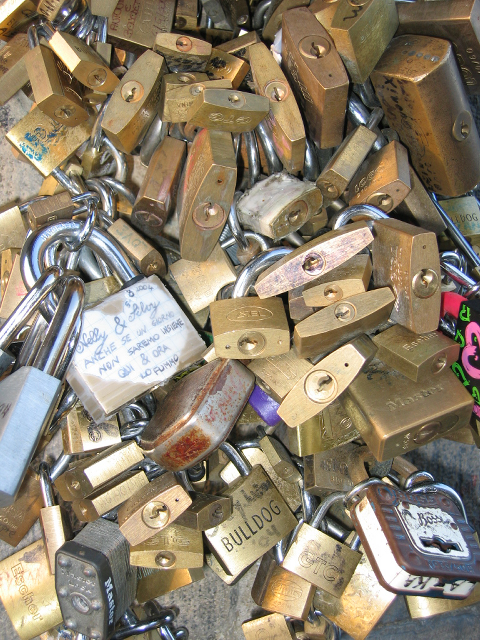
\includegraphics[scale=0.35]{images/candados.png}
    \caption{candados.bmp}
    
\end{figure}

\subsubsection{lennon}
He seleccionado esta imagen debido a su fondo uniforme, lo cual permitirá al compresor aprovecharlo y lograr un buen ratio de compresión. Además, la imagen contiene elementos detallados, como las gafas y el micrófono, que resultará interesante analizar en términos de cómo conservan sus detalles en diferentes configuraciones de los compresores.\\

La imagen es de $1375\times1031$ píxeles y ocupa 4.05MB. Se trata de una imagen bastante grande, puesto que creo que resultará interesante extraer datos sobre el desempeño de los compresores en imágenes de distintos tamaños (grandes y pequeños).\\

\begin{figure}[H]
    \centering
    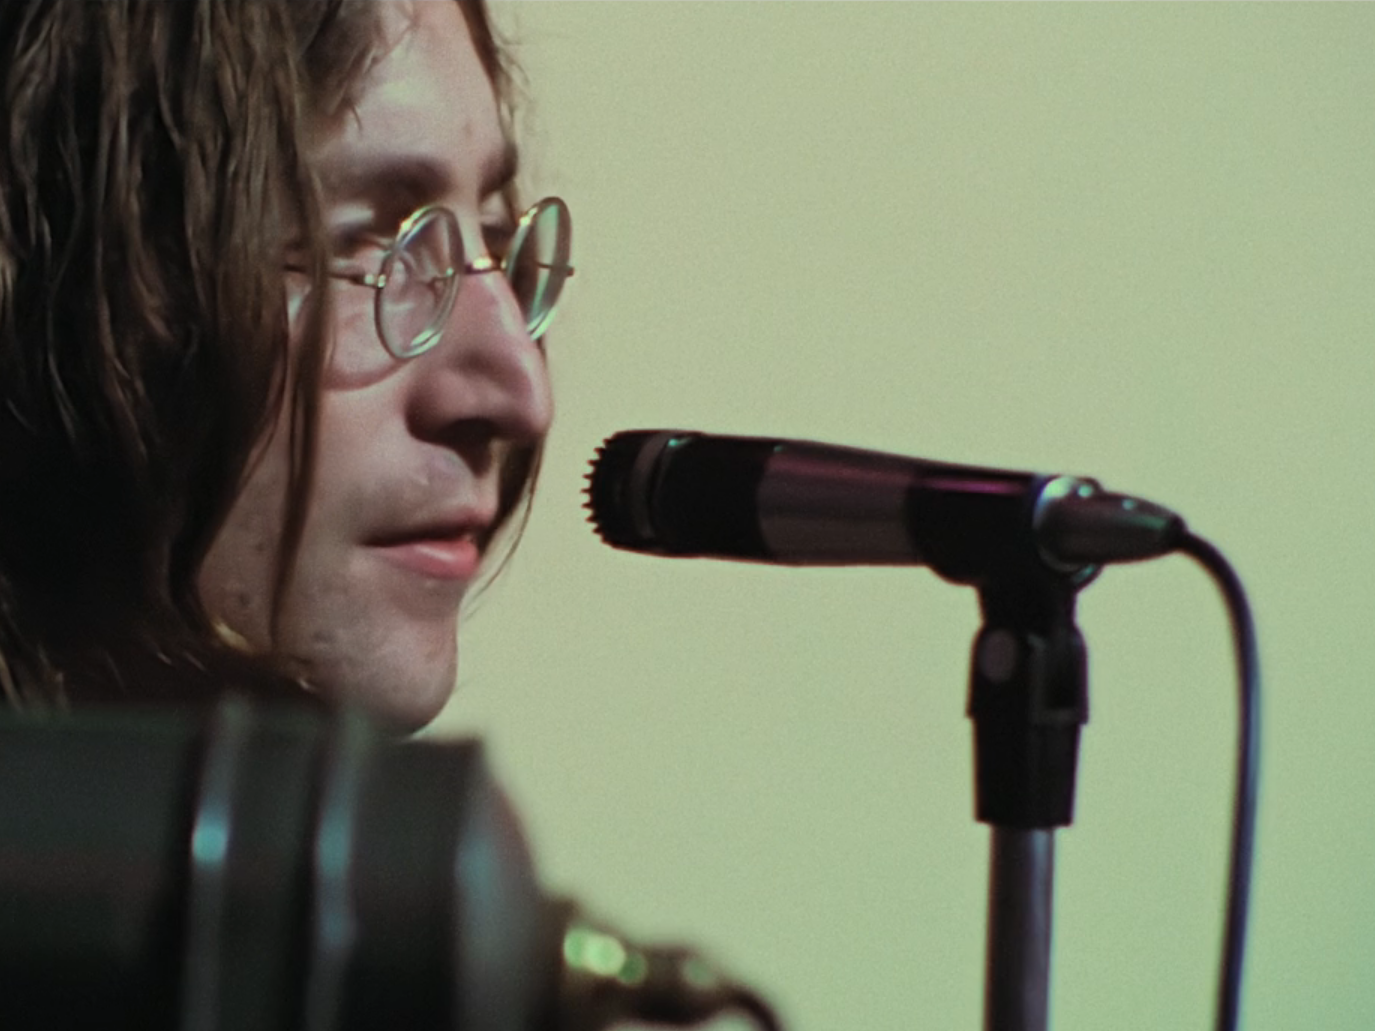
\includegraphics[scale=0.2]{images/lennon.png}
    \caption{lennon.bmp}
    
\end{figure}

\break
\subsubsection{lena}
Esta imagen ha sido ampliamente utilizada en el campo de la compresión de imágenes como referencia para evaluar el desempeño de los algoritmos compresores, y es probablemente la imagen más famosa en este campo de investigación.\\ 

Es una elección interesante debido a las áreas con alto nivel de detalle, como el cabello y los ojos, y su fondo no uniforme pero relativamente plano. La hemos incluido en nuestro estudio debido a su relevancia histórica y por ser un estándar ampliamente reconocido en la industria.\\

Como hipótesis inicial, a pesar de ser una imagen en blanco y negro sin transiciones abruptas de color, considero que los resultados obtenidos no serán óptimos debido a la gran cantidad de detalles que contiene. Es probable que no sea posible alcanzar tasas de compresión elevadas sin perder una considerable cantidad de información visual.\\

La imagen es de $512\times512$ píxeles y ocupa 768KB.\\

\begin{figure}[H]
    \centering
    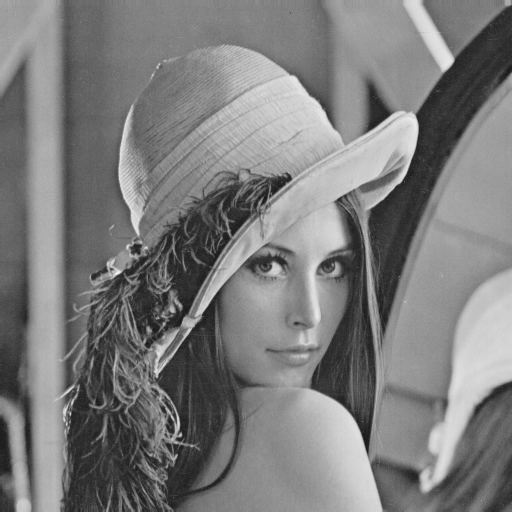
\includegraphics[scale = 0.40]{images/lena.png}
    \caption{lena.bmp. Fuente:\cite{NYU-SampleData}}
    
\end{figure}

\break
\subsubsection{mandrill}
La siguiente imagen se ha obtenido de la base de datos de imágenes proporcionada por la USC (University of Southern California) \cite{USCSIPI-Database}.\\

La imagen muestra un primer plano de la cabeza de un mandril, con muchos detalles. Como en el caso anterior, se utiliza frecuentemente como imagen de referencia para evaluar distintos algoritmos de compresión.\\

La imagen es interesante debido a que presenta una gran variedad de colores (desde colores vivos a colores más apagados, nos permitirá ver cómo de bien se preserva el color), así como de texturas (distintas texturas del pelo muy complejas, textura más plana y regular de la piel, etc.). En definitiva, se trata de una imagen de la que esperamos obtener información significativa sobre el desempeño de los dos compresores.\\ 

Tiene unas diemensiones de $512\times512$ píxeles y ocupa 768KB.\\

\begin{figure}[H]
    \centering
    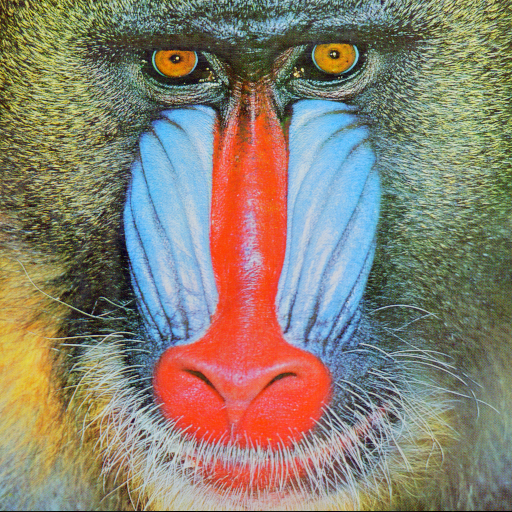
\includegraphics[scale = 0.40]{images/mandrill.png}
    \caption{mandrill.bmp}
\end{figure}

\break
\subsubsection{noise} \label{noisepre}
Esta imagen ha sido generada utilizando un sencillo programa en Python, donde los píxeles de colores se han asignado de manera aleatoria. En este caso, se espera que los resultados de la compresión sean muy deficientes, ya que los compresores aprovechan la correlación espacial para lograr una mayor compresión. Sin embargo, en esta imagen, dicha correlación es prácticamente inexistente, lo que implica que para mantener la similitud visual, se requerirán prácticamente todos los coeficientes de la transformada de coseno discreta (DCT), lo que resultará en tasas de compresión extremadamente bajas.\\

El objetivo de incluir esta imagen es evaluar el rendimiento de cada compresor ante un caso altamente desfavorable. Posteriormente, se compararán estos resultados con los obtenidos en un caso favorable, con el fin de destacar la importancia de la correlación espacial en el rendimiento de estos compresores.\\

La imagen es de $320\times240$ píxeles y ocupa 225KB.\\

\begin{figure}[H]
    \centering
    
\includegraphics[scale = 0.8]{images/noise.png}
    \caption{noise.bmp}
    
\end{figure}

\break
\subsubsection{pattern}
En el caso de esta imagen, debido a su patrón repetitivo, se espera que la transformada de coseno discreta (DCT) pueda aprovechar la redundancia espacial presente en la imagen. Además, la codificación Huffman podría ser eficiente en la compresión de los elementos más repetitivos dentro del patrón. Con base en esta consideración, mi hipótesis es que esta imagen debería alcanzar altos niveles de compresión sin perder significativamente el parecido visual con la imagen original.\\

Será interesante realizar una comparación entre los resultados obtenidos en esta imagen y los de la imagen anterior que carecía de correlación espacial. Esto nos permitirá analizar y contrastar los efectos de la correlación espacial en los resultados de compresión (\ref{noisepre}).\\

La imagen es de $320\times240$ píxeles y ocupa 225KB. La he escogido del mismo tamaño que la anterior para poder comparar ambas mejor.\\

\begin{figure}[H]
    \centering
    
\includegraphics[scale = 0.8]{images/pattern.png}
    \caption{pattern.bmp}
    
\end{figure}

\break
\subsubsection{color\_bars}
Cuando una imagen contiene líneas verticales, estas líneas se traducen en coeficientes DCT con valores altos en las frecuencias verticales. En otras palabras, estas líneas generan energía concentrada en las componentes de alta frecuencia vertical de la imagen. Como resultado, muchos coeficientes en esas frecuencias tras realizar la DCT tendrán valores significativos, mientras que los coeficientes en otras frecuencias pueden tener valores cercanos a cero. Además, como solamente hay 8 líneas verticales anchas, los valores deberían concentrarse todavía más en algunos pocos componentes. De esta manera, durante la cuantización se podrá asignar a estos componentes etiquetas más pequeñas, para conseguir resultados de compresión muy buenos.\\

Mediante este ejemplo, busco evaluar un caso extremadamente favorable para los compresores. Se espera que esta imagen alcance las tasas de compresión más elevadas entre todas las que se están probando, con una diferencia visual prácticamente imperceptible en comparación con la imagen original para la mayoría de los factores de calidad evaluados\\  

La imagen es de $640\times480$ píxeles y ocupa 900KB.\\
 
\begin{figure}[H]
    \centering
    
\includegraphics[scale=0.65]{images/color_bars.png}
    \caption{color\_bars.bmp}
    
\end{figure}

\break
\subsubsection{explorer}
Esta imagen muestra un fragmento del explorador de archivos de Microsoft Windows 10, que contiene tanto texto como iconos. En nuestro análisis, nos enfocaremos en evaluar si el texto, los botones y otros elementos como los iconos se mantienen legibles y conservan un nivel adecuado de detalle.\\

Mediante este ejemplo, buscamos examinar el comportamiento de los compresores en una imagen que presenta texto sobre un fondo plano. Las diferencias visuales pueden tener un impacto significativo en la legibilidad del texto, por lo que resulta especialmente interesante estudiar cómo los compresores afectan a esta característica. Además, la imagen también contiene iconos pequeños, los cuales deseamos preservar con un alto nivel de detalle.\\

A primera vista, el fondo plano nos podría llevar a pensar que se obtendrán buenos resultados de compresión. Sin embargo, debido a la fuerte condición de que el texto debe ser legible, resulta difícil realizar una estimación precisa sobre los resultados obtenidos.\\

La imagen es de $720\times320$ píxeles y ocupa 675KB.\\

\begin{figure}[H]
    \centering
    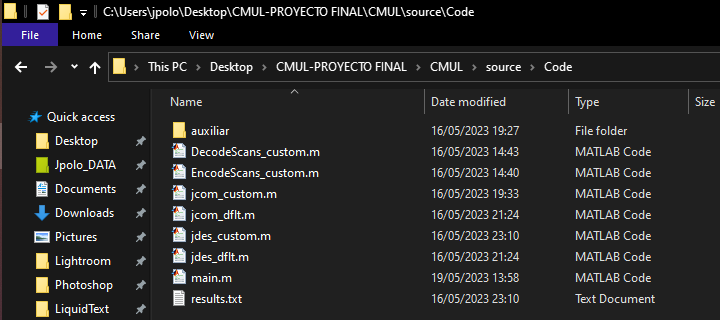
\includegraphics[scale=0.5]{images/explorer.png}
    \caption{explorer.bmp}
    
\end{figure}


\break
\subsubsection{gradient}
En la imagen vemos una progresión de colores que se produce de forma suave y sin cambios bruscos entre zonas de distinto color.\\

Creo que esta característica es relevante e interesante, ya que se encuentra comúnmente en muchas fotografías del mundo real, como los tonos del cielo o los elementos grandes que presentan distintos tonos de color según la iluminación. En estas situaciones, los cambios de color se producen de manera gradual en lugar de brusca. Como hipótesis inicial, creo que se irán formando distintas regiones del mismo color, es decir, que los colores se ``unifiquen'' en diferentes regiones. Sin embargo, debido a que el cambio de color es suave, considero que se podrán obtener buenos resultados de compresión sin sacrificar calidad visual.\\ 

Mediante esta imagen, tenemos como objetivo analizar el fenómeno que ocurre al comprimir un patrón de gradación de color de forma aislada, sin la presencia de otros elementos en la imagen que puedan condicionar este análisis. Los resultados obtenidos en este análisis nos permitirán extrapolarlos posteriormente a otras imágenes que contengan regiones de color con características similares.\\

La imagen es de $300\times300$ píxeles y ocupa 263KB.\\

\begin{figure}[H]
    \centering
    
\includegraphics{images/gradient.png}
    \caption{gradient.bmp}
    
\end{figure}

\break
\subsubsection{color\_shapes}
En esta imagen, podemos observar grandes zonas que comparten el mismo color, separadas por fronteras diagonales. Considero que esta imagen resulta interesante para analizar el comportamiento de los compresores con respecto a las líneas diagonales que delimitan las diferentes regiones. Esto se debe a que, al eliminar las componentes menos significativas durante el proceso de transformada de coseno discreta (DCT), se puede perder detalle visual, lo que podría ocasionar que las líneas diagonales presenten una apariencia ``escalonada''.\\

Basado en esta consideración, planteo la hipótesis de que los cambios drásticos entre las regiones en la imagen provocarán una pérdida significativa de calidad visual en las líneas diagonales, incluso con factores de compresión bajos. En consecuencia, se espera que los resultados de la compresión no sean muy buenos en este caso.\\

La imagen es de $320\times240$ píxeles y ocupa 225KB.\\

\begin{figure}[H]
    \centering
    
\includegraphics[scale=0.8]{images/cshapes.png}
    \caption{cshapes.bmp}
    
\end{figure}

\break
\subsubsection{x-ray}
La siguiente imagen es una radiografía que he digitalizado yo mismo.\\

Como planteaba en la introducción, uno de los ámbitos donde la compresión de imágenes eficaz puede tener mucha importancia es en el ámbito médico-sanitario.\\

En este ejemplo destacan por un lado la gran cantidad de detalles de los huesos que deben preservarse de la mejor manera posible, y por otro la información complementaria y la escala de medida indicadas como texto. Además, las imágenes de los huesos presentan un regiones con color uniforme y cambios suaves en contraste con la región negra prácticamente uniforme del fondo.\\

De esta manera, la imagen combina muchas de las características interesantes para el análisis mencionadas en las imágenes anteriores en un caso de ejemplo que podemos considerar bastante realista.\\

La imagen es de $1169\times654$ píxeles y ocupa $2.18$MB

\begin{figure}[H]
    \centering
    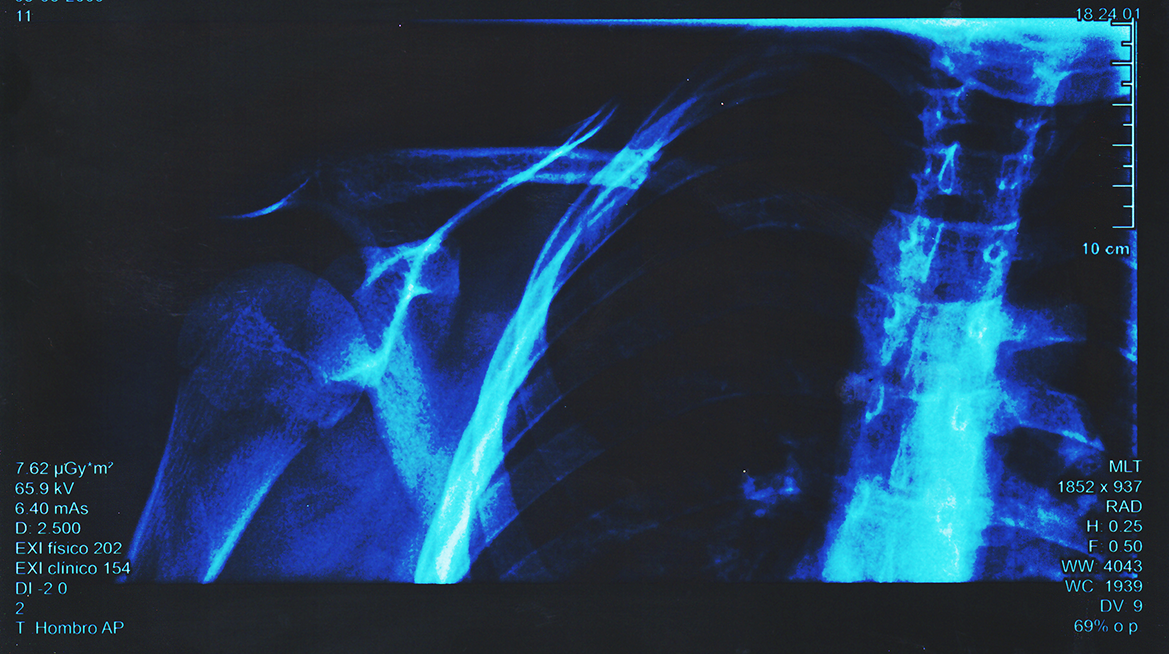
\includegraphics[scale = 0.35]{images/xray.png}
    \caption{x- ray.bmp}
\end{figure}

\break

\newpage
\section{Resultados experimentales}
En esta sección, analizaremos los resultados obtenidos a partir de los experimentos realizados. Comenzaremos con el estudio cualitativo, seguido del estudio cuantitativo.

El estudio cualitativo se enfoca en el parecido visual entre las imágenes originales y las comprimidas. Evaluaré la preservación de los detalles, la legibilidad del texto, la calidad de los colores y la apariencia general de las imágenes. Realizaré una comparación y señalaré cualquier diferencia notable. Cabe destacar que este análisis está sujeto a la interpretación personal.\\

Posteriormente, realizaremos el estudio cuantitativo, el cual se basa en las métricas definidas en la sección \ref{metricasCuant}. Calcularemos el Ratio de Compresión (\textit{RC}), el Signal-to-Noise Ratio (\textit{SNR}) y el Error Cuadrático Medio (\textit{MSE}) para cada imagen y para ambos compresores utilizados. Estas métricas nos proporcionarán una medida cuantitativa del desempeño de los compresores y nos permitirán comparar los resultados obtenidos.\\

Es importante tener en cuenta que, aunque el análisis cuantitativo nos brinda información objetiva, no debemos descartar la importancia del análisis cualitativo. Ambos enfoques son complementarios y nos ayudarán a evaluar de manera integral los resultados obtenidos en nuestros experimentos.\\

\subsection{Estudio cualitativo}
Debido a la cantidad considerable de datos generados durante los experimentos, hemos realizado un análisis preliminar de los resultados y decidido focalizar nuestra discusión en los valores del parámetro de calidad $50$, $100$ y $200$. Estos valores representan niveles de compresión baja, media y alta, respectivamente. No obstante, en casos específicos donde sea relevante, también mencionaremos otros valores.\\

Consideramos que estos valores seleccionados proporcionan una visión representativa de los resultados obtenidos y nos permitirán analizar el impacto de la compresión en las imágenes.\\

Cabe destacar que el proceso de estudio cualitativo se realiza sobre los ficheros de las imágenes obtenidas. Aquí simplemente se muestran en un tamaño reducido con fines orientativos, recomendamos consultar los ficheros correspondientes.\\

Los ficheros de las imágenes resultantes se encuentran en \textit{\textbackslash source\textbackslash Images\textbackslash decoded\_dflt} en el caso de las imágenes del compresor por defecto, y en \textit{\textbackslash source\textbackslash Images\textbackslash decoded\_custom} en el caso del compresor customizado.

\subsubsection{candados}
Primero se muestra la imagen original para tener una referencia:
\begin{figure}[H]
    \centering
    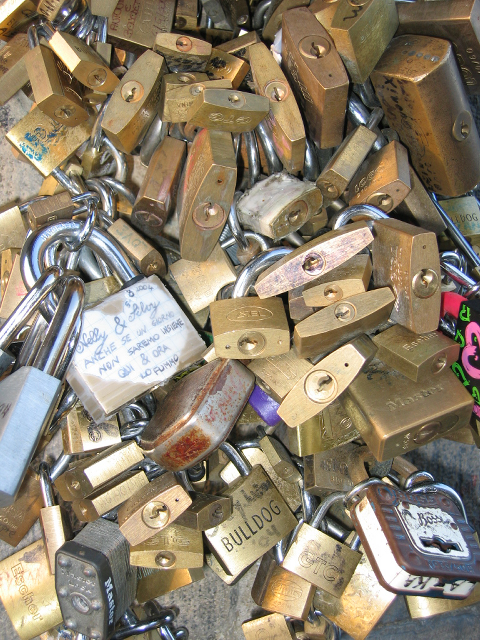
\includegraphics[width=0.20\textwidth]{images/candados.png}
    \caption[Referencia - candados]{Imagen original de referencia.}
    \label{fig:top_candados}
\end{figure}
    \vspace{0.5cm}

Imágenes resultantes:
\begin{figure}   [H]
    \begin{subfigure}{0.20\textwidth}
        \centering
        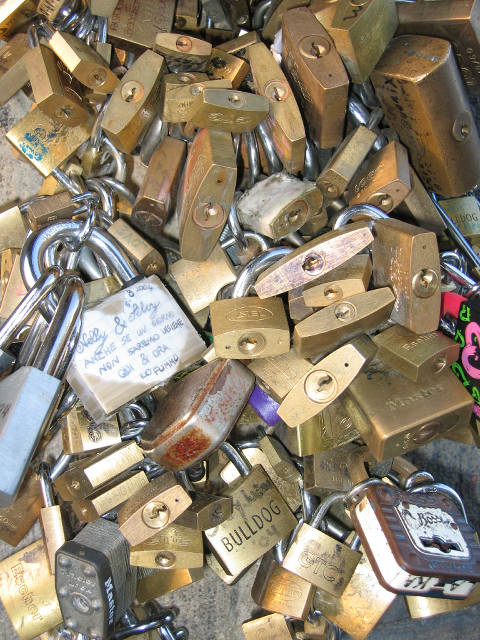
\includegraphics[width=\linewidth]{dflt/candados_Q50_dec_dflt.png}
        \caption{CaliQ=50.}
        
    \end{subfigure}
    \hfill
    \begin{subfigure}{0.20\textwidth}
        \centering
        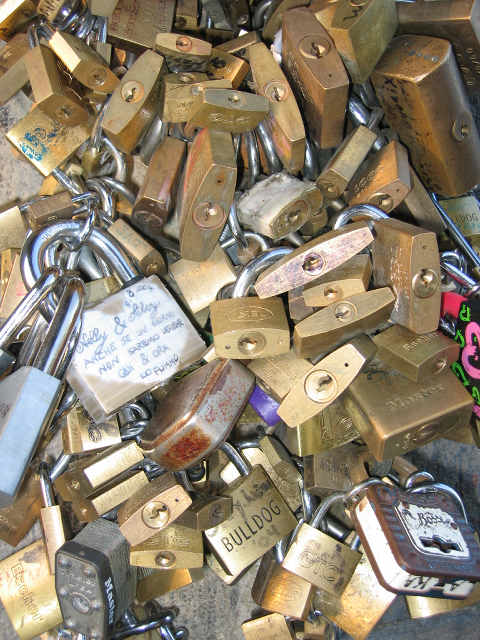
\includegraphics[width=\linewidth]{dflt/candados_Q100_dec_dflt.png}
        \caption{CaliQ=100.}
        
    \end{subfigure}
    \hfill
    \begin{subfigure}{0.20\textwidth}
        \centering
        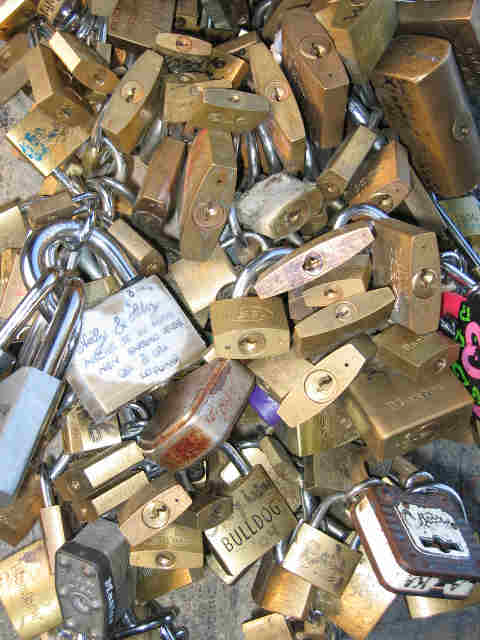
\includegraphics[width=\linewidth]{dflt/candados_Q250_dec_dflt.png}
        \caption{CaliQ=200.}
        
    \end{subfigure}
    
    
    \caption[Resultados experimentales - candado]{Resultados experimentales de la compresión de la imagen \textit{candados.bmp}.}
    \label{fig:candados_cuali}
\end{figure}

En la figura \ref{fig:top_candados}, vemos la imagen original que servirá de referencia. En la figura \ref{fig:candados_cuali} vemos las imágenes obtenidas como resultado de la compresión, en la primera fila por el compresor por defecto y en la segunda por el compresor customizado. Este formato será el mismo para el resto de imágenes.\\

Como observación inicial, podemos destacar un fenómeno interesante: Los resultados visuales para el compresor por defecto y el compresor customizado son prácticamente idénticos. Esto sucederá también con el resto de imágenes, de forma que se espera que la diferencia, si es que la hay, sea en el análisis cuantitativo.\\

Centrándonos en la imagen, con factor de calidad 50 no se aprecian diferencias muy significativas respecto a la original, como diferencia más notable se aprecia la textura de los candados, que empieza a verse más pixelada, así como los bordes de las marcas y las letras en las que se ve un efecto más pixelado. En cualquier caso estos detalles son muy sutiles.\\

Con factor de calidad 100 las diferencias anteriores se acentúan de forma moderada, y se ven claramente zonas en las que se forman ``manchas'' de píxeles. Esto es más notable en las zonas que no tienen un color uniforme. Las letras escritas sobre el candado grande (azul sobre fondo blanco) se distinguen pero con dificultad.\\

En el factor de calidad 200 las diferencias son enormes. La imagen adquiere una textura pixelada (se aprecian grandes bloques de píxeles que componen la imagen). Hay además fallos de color, porque aparecen colores y tonalidades donde antes parecía un color casi uniforme, y las letras no son distinguibles de ninguna manera. Consideramos que este resultado no es ya adecuado visualmente.\\

En este caso considero que el factor de calidad 100 es el más adecuado, puesto que aunque presenta más diferencias que el factor 50, la imagen se sigue viendo natural y los elementos como las letras continúan siendo visibles. El efecto de la pixelación todavía no es tan notable alterando bordes y colores y lo considero un resultado adecuado.\\



\subsubsection{lennon}
Primero se muestra la imagen original para tener una referencia:
\begin{figure}[H]
    \centering
    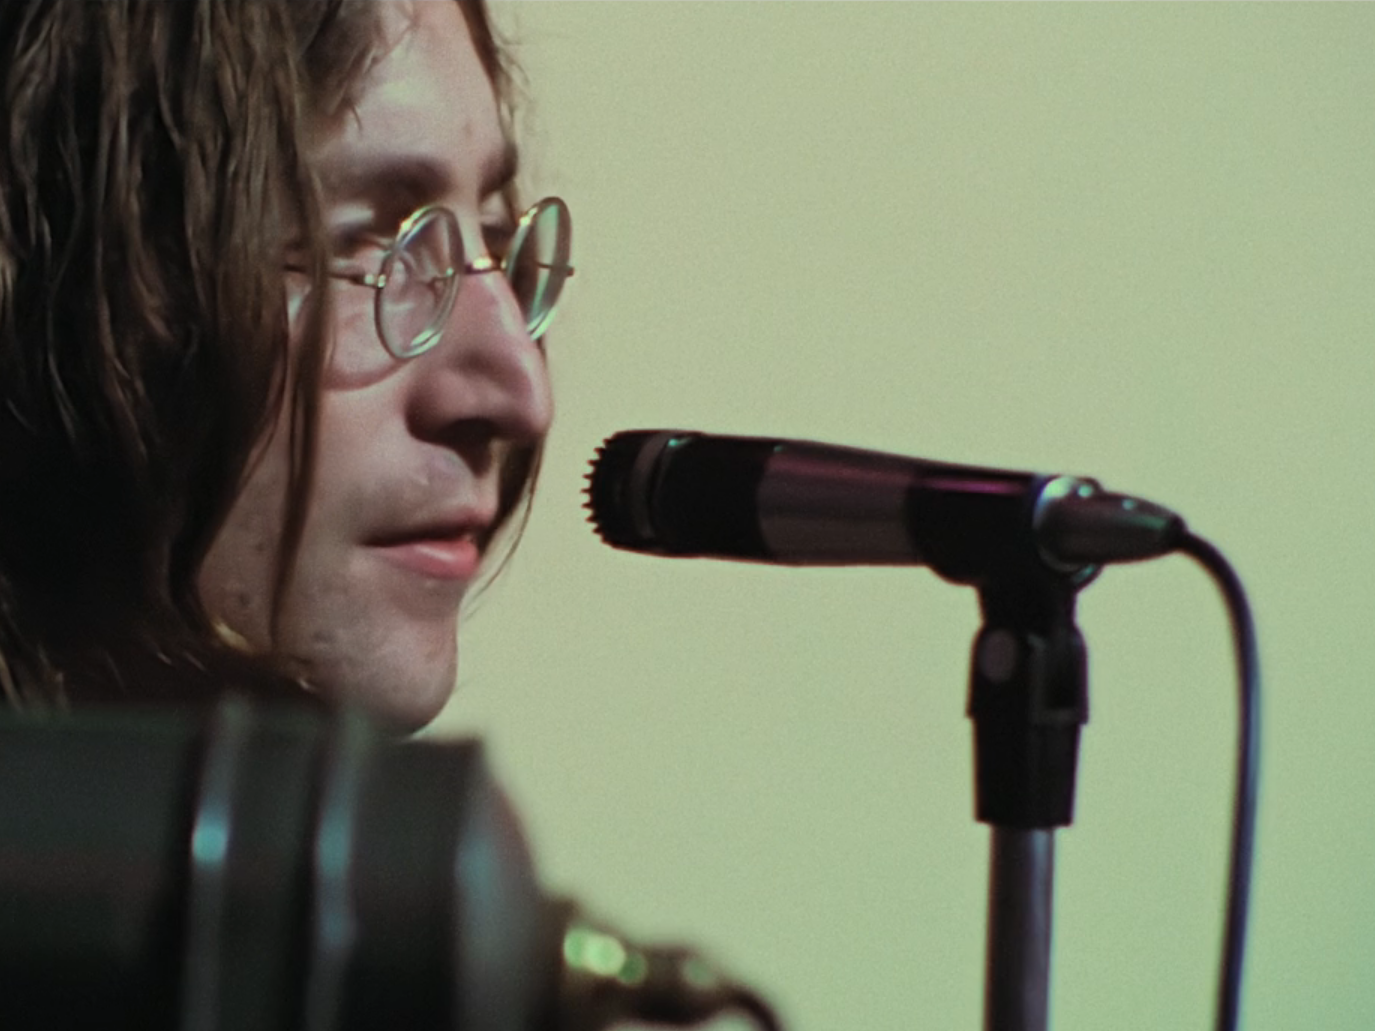
\includegraphics[width=0.30\textwidth]{images/lennon.png}
    \caption[Referencia - lennon]{Imagen original de referencia.}
    
 \end{figure}   
    \vspace{0.5cm}
    
Imágenes resultantes:
\begin{figure}   [H]   
    \begin{subfigure}{0.30\textwidth}
        \centering
        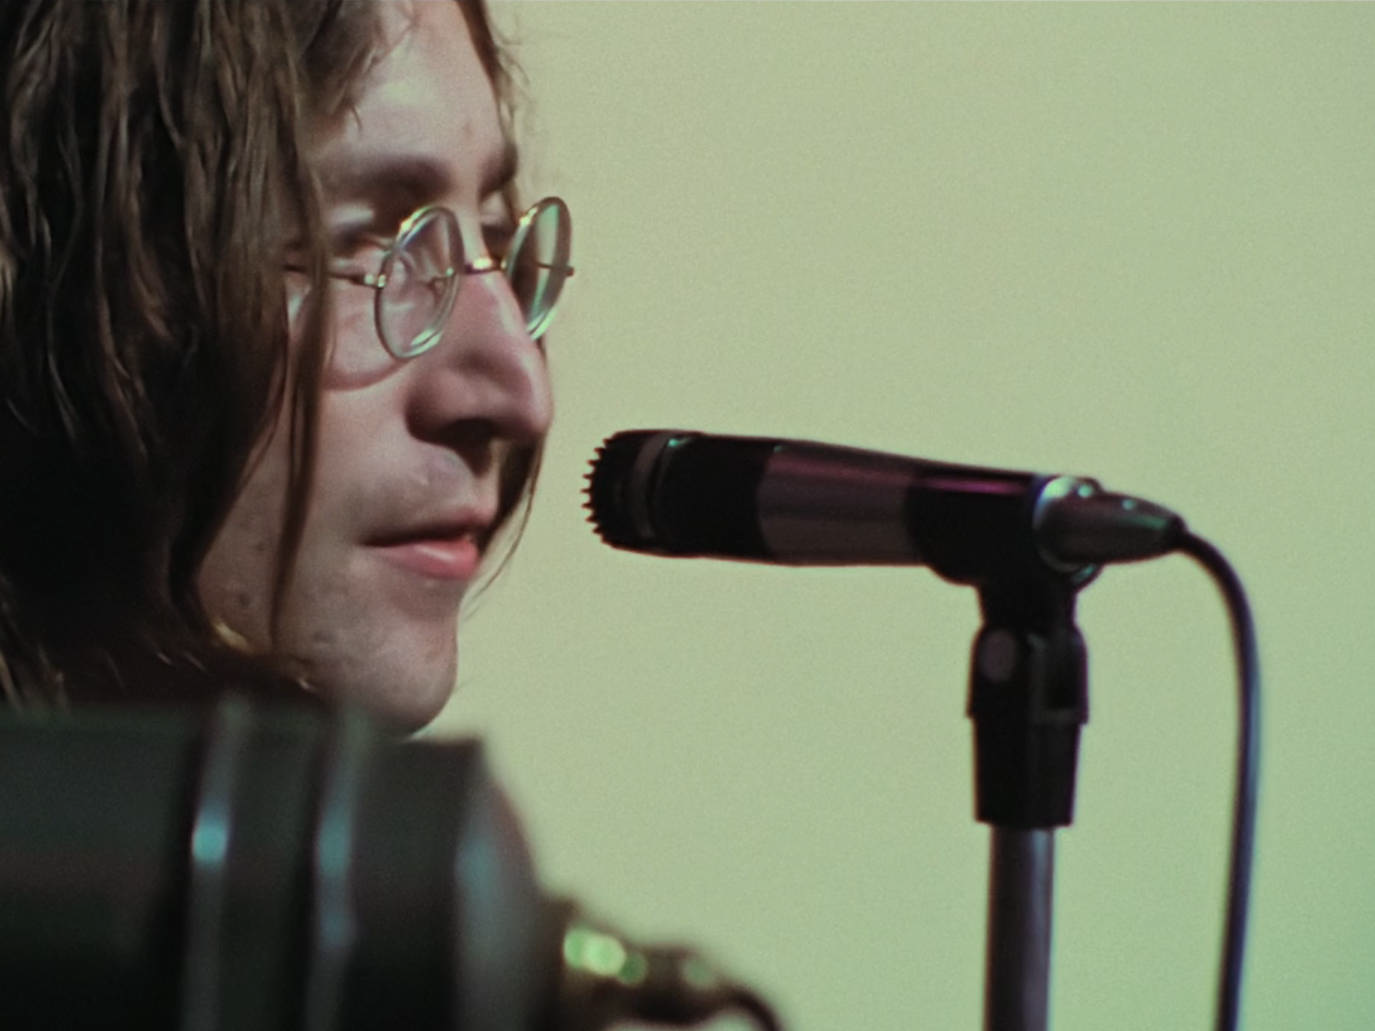
\includegraphics[width=\linewidth]{dflt/lennon_Q50_dec_dflt.png}
        \caption{CaliQ=50.}
        
    \end{subfigure}
    \hfill
    \begin{subfigure}{0.30\textwidth}
        \centering
        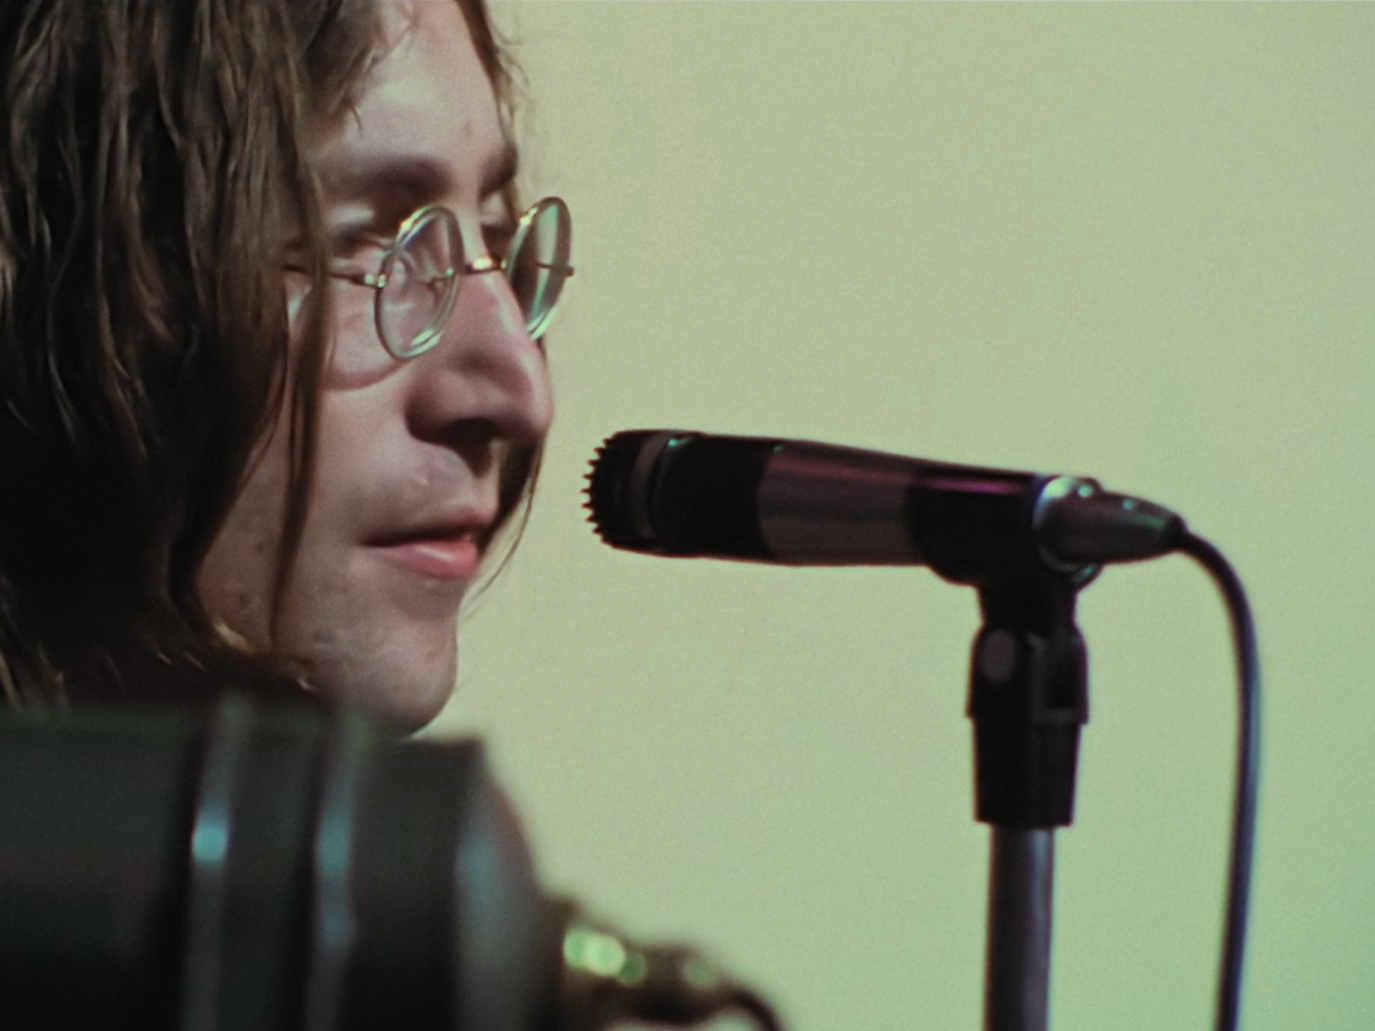
\includegraphics[width=\linewidth]{dflt/lennon_Q100_dec_dflt.png}
        \caption{CaliQ=100.}
        
    \end{subfigure}
    \hfill
    \begin{subfigure}{0.30\textwidth}
        \centering
        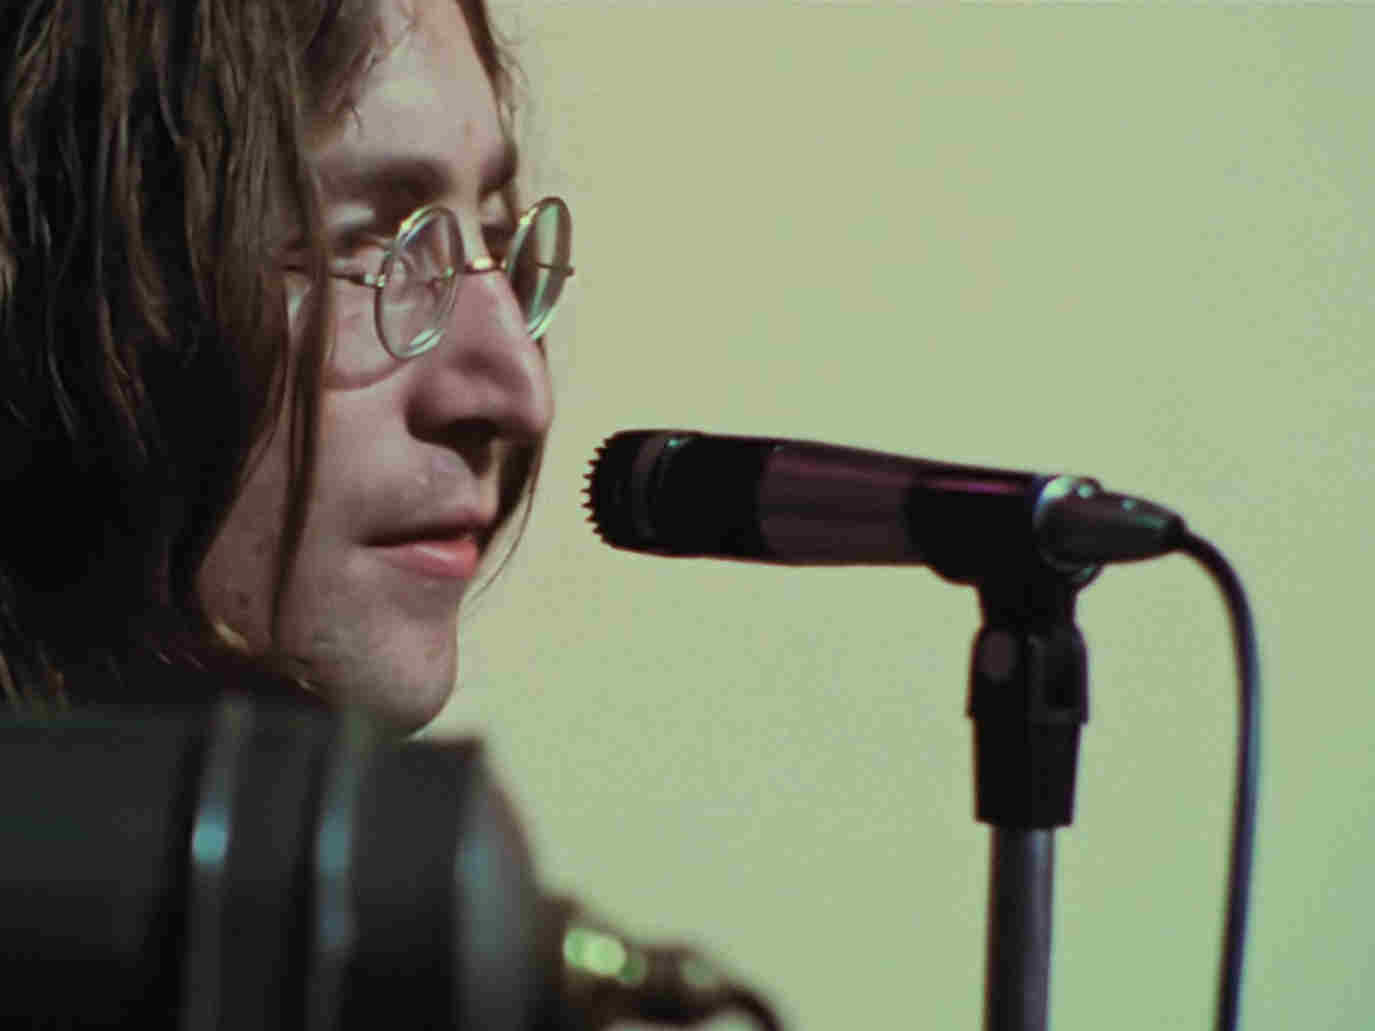
\includegraphics[width=\linewidth]{dflt/lennon_Q250_dec_dflt.png}
        \caption{CaliQ=200.}
        
    \end{subfigure}

    
    \caption[Resultados experimentales - lennon]{Resultados experimentales de la compresión de la imagen \textit{lennon.bmp}.}
    
\end{figure}

En esta imagen no aprecio diferencias muy notables entre los resultados con factor 50 y con factor 100. Los elementos principales de la imagen se siguen apreciando prácticamente igual, quizás debido a que la imagen original no tenía una gran cantidad de enfoque y una textura granulosa característica de las imágenes analógicas más antiguas (cuando más se notan las diferencias es cuando la imagen original tiene un enfoque muy nítido y texturas muy regulares, porque es de lo primero que se va perdiendo al comprimir la imagen). El fondo de la imagen empieza a unificarse en bloques del mismo color, pero al ser muy regular en la imagen original apenas sí se aprecia. Con factor 200 la imagen empeora notablemente. Adquiere una textura pixelada , aparecen manchas en la cara y el fondo se ve como grandes manchas de píxeles con una transición abrupta entre regiones. Elementos como el micrófono han perdido casi todos sus detalles, adquiriendo una textura plana.\\

Por estas razones escogeré el factor 100.


\subsubsection{lena}
Primero se muestra la imagen original para tener una referencia:
\begin{figure}[H]
    \centering
    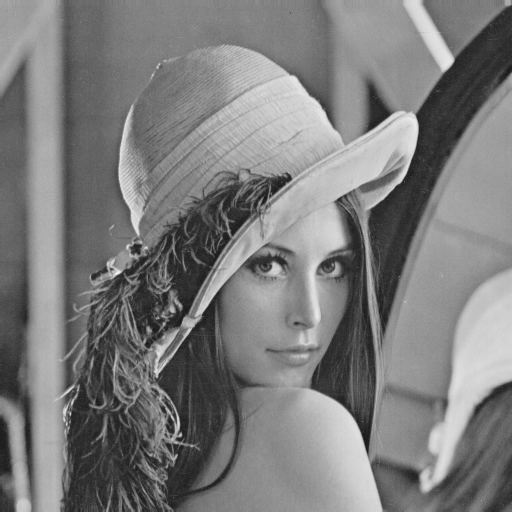
\includegraphics[width=0.30\textwidth]{images/lena.png}
    \caption[Referencia - lena]{Imagen original de referencia.}
    
\end{figure}
    
    \vspace{0.5cm}
    
Imágenes resultantes:
\begin{figure}   [H]
    \begin{subfigure}{0.30\textwidth}
        \centering
        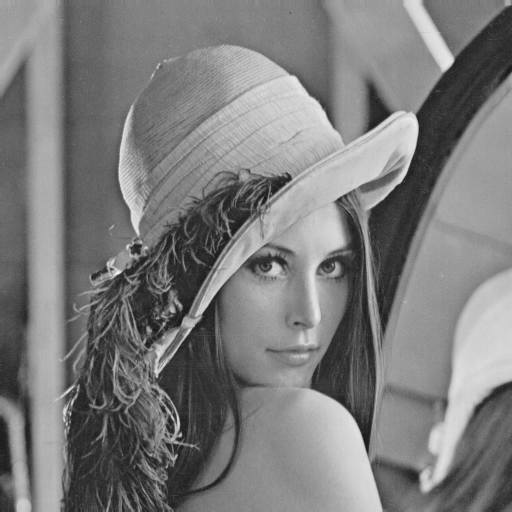
\includegraphics[width=\linewidth]{dflt/lena_Q50_dec_dflt.png}
        \caption{CaliQ=50.}
        
    \end{subfigure}
    \hfill
    \begin{subfigure}{0.30\textwidth}
        \centering
        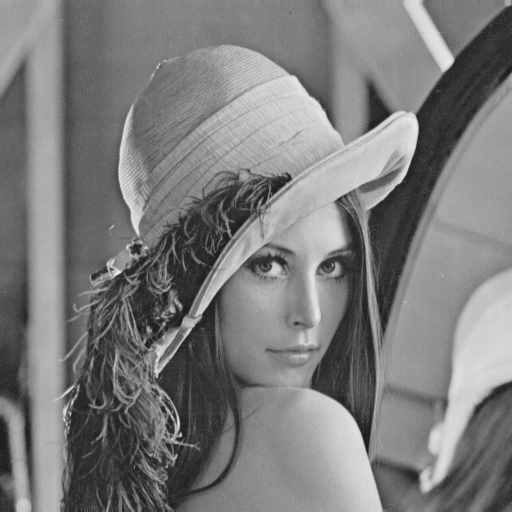
\includegraphics[width=\linewidth]{dflt/lena_Q100_dec_dflt.png}
        \caption{CaliQ=100.}
        
    \end{subfigure}
    \hfill
    \begin{subfigure}{0.30\textwidth}
        \centering
        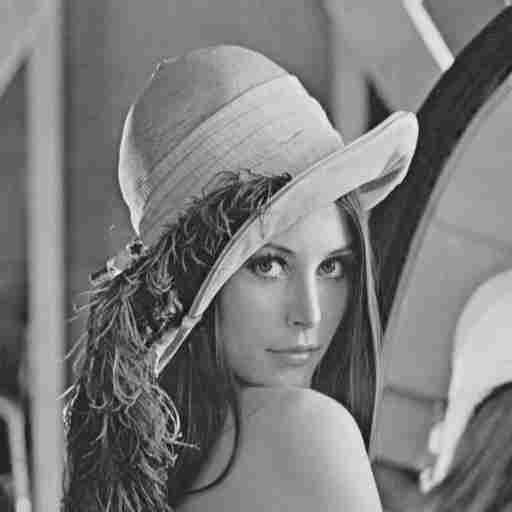
\includegraphics[width=\linewidth]{dflt/lena_Q250_dec_dflt.png}
        \caption{CaliQ=200.}
        
    \end{subfigure}
    
    \caption[Resultados experimentales - lena]{Resultados experimentales de la compresión de la imagen \textit{lena.bmp}.}
    
\end{figure}

En esta imagen los resultados son bastante buenos, y la diferencia entre el factor 50 y el factor 100 es mínima, y apenas se pierden detalles respecto a la imagen original. Con factor 200 la imagen adquiere la textura pixelada que ya hemos comentado en las imágenes anteriores y en el fondo aparecen manchas uniformes muy apreciables.\\ 

En este caso elegiré también el factor 100.

\subsubsection{mandrill}
Primero se muestra la imagen original para tener una referencia:
\begin{figure}[H]
    \centering
    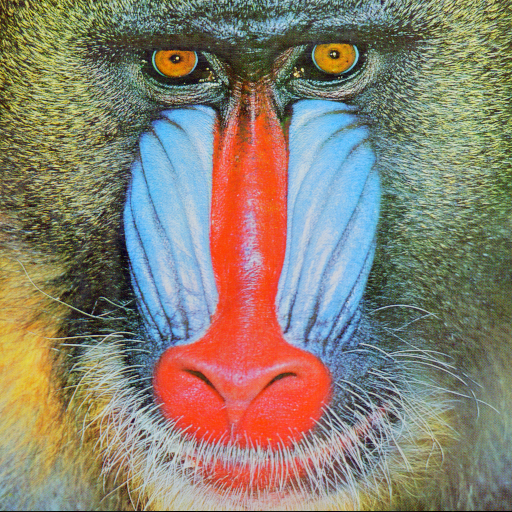
\includegraphics[width=0.30\textwidth]{images/mandrill.png}
    \caption[Referencia - mandrill]{Imagen original de referencia.}
    
\end{figure}
    
    \vspace{0.5cm}

Imágenes resultantes:
\begin{figure}   [H]
    \begin{subfigure}{0.30\textwidth}
        \centering
        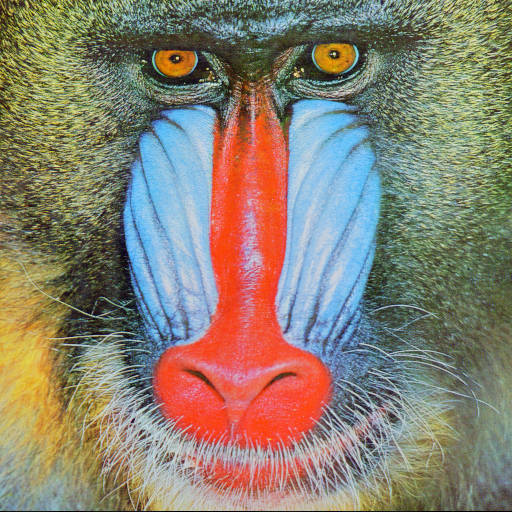
\includegraphics[width=\linewidth]{dflt/mandrill_Q50_dec_dflt.png}
        \caption{CaliQ=50.}
        
    \end{subfigure}
    \hfill
    \begin{subfigure}{0.30\textwidth}
        \centering
        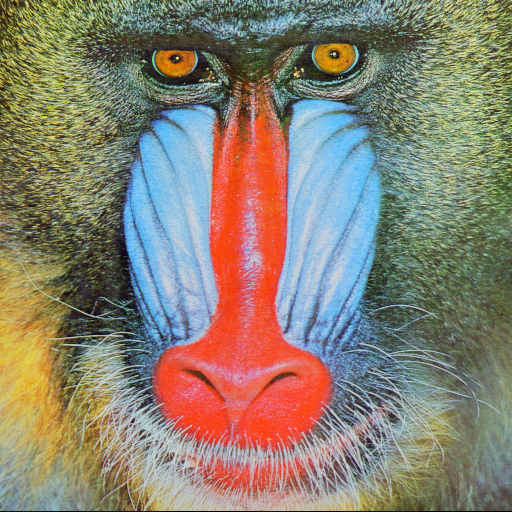
\includegraphics[width=\linewidth]{dflt/mandrill_Q100_dec_dflt.png}
        \caption{CaliQ=100.}
        
    \end{subfigure}
    \hfill
    \begin{subfigure}{0.30\textwidth}
        \centering
        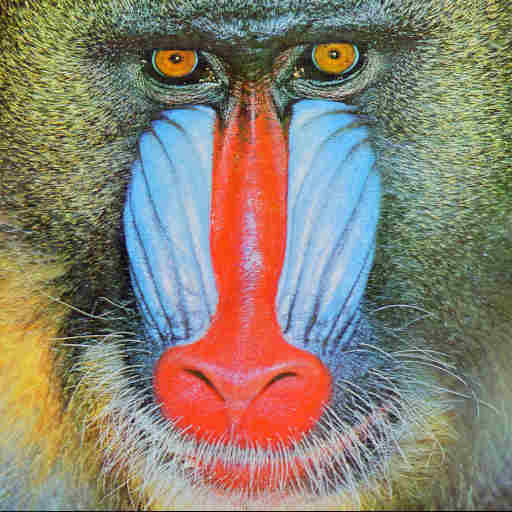
\includegraphics[width=\linewidth]{dflt/mandrill_Q250_dec_dflt.png}
        \caption{CaliQ=200.}
        
    \end{subfigure}
    
    \caption[Resultados experimentales - mandrill]{Resultados experimentales de la compresión de la imagen \textit{mandrill.bmp}.}
    
\end{figure}

En esta imagen enseguida se aprecia la pérdida de calidad incluso en los niveles bajos de compresión. Con CaliQ=100, las texturas de la imagen pierden mucho detalle, especialmente en las zonas del pelo en las esquinas, y la imagen se ve en general ``desenfocada'' respecto a la original. Los colores, sin embargo, se preservan sorprendentemente bien, incluso en las zonas con cambios bruscos de color.\\

En este caso elegiré el factor CaliQ=50, por la pérdida de detalle en niveles superiores.\\


\subsubsection{noise}
Primero se muestra la imagen original para tener una referencia:
\begin{figure}[H]
    \centering
    
\includegraphics[width=0.30\textwidth]{images/noise.png}
    \caption[Referencia - noise]{Imagen original de referencia.}
    
\end{figure}
    
    \vspace{0.5cm}

Imágenes resultantes:
\begin{figure}   [H]
    \begin{subfigure}{0.30\textwidth}
        \centering
        
\includegraphics[width=\linewidth]{dflt/noise_Q50_dec_dflt.png}
        \caption{CaliQ=50.}
        
    \end{subfigure}
    \hfill
    \begin{subfigure}{0.30\textwidth}
        \centering
        
\includegraphics[width=\linewidth]{dflt/noise_Q100_dec_dflt.png}
        \caption{CaliQ=100.}
        
    \end{subfigure}
    \hfill
    \begin{subfigure}{0.30\textwidth}
        \centering
        
\includegraphics[width=\linewidth]{dflt/noise_Q250_dec_dflt.png}
        \caption{CaliQ=200.}
        
    \end{subfigure}
    
    \caption[Resultados experimentales - noise]{Resultados experimentales de la compresión de la imagen \textit{noise.bmp}.}
    
\end{figure}

Esta imagen es un poco difícil de analizar debido a que no hay formas ni contornos reconocibles. No aprecio ninguna diferencia entre el factor 50 y el factor 100. En el factor 200 ya noto como la imagen se agrupa en bloques de píxeles bien diferenciados. Será interesante ver las diferencias cuantitativas entre los dos primeros factores de calidad.\\

Elijo el factor 100.


\subsubsection{pattern}
Primero se muestra la imagen original para tener una referencia:
\begin{figure}[H]
    \centering
    
\includegraphics[width=0.30\textwidth]{images/pattern.png}
    \caption[Referencia - pattern]{Imagen original de referencia.}
    
\end{figure}
    \vspace{0.5cm}

Imágenes resultantes:
\begin{figure}[H]

    \begin{subfigure}{0.30\textwidth}
        \centering
        
\includegraphics[width=\linewidth]{dflt/pattern_Q50_dec_dflt.png}
        \caption{CaliQ=50.}
        
    \end{subfigure}
    \hfill
    \begin{subfigure}{0.30\textwidth}
        \centering
        
\includegraphics[width=\linewidth]{dflt/pattern_Q100_dec_dflt.png}
        \caption{CaliQ=100.}
        
    \end{subfigure}
    \hfill
    \begin{subfigure}{0.30\textwidth}
        \centering
        
\includegraphics[width=\linewidth]{dflt/pattern_Q250_dec_dflt.png}
        \caption{CaliQ=200.}
        
    \end{subfigure}
    
    \caption[Resultados experimentales - pattern]{Resultados experimentales de la compresión de la imagen \textit{pattern.bmp}.}
    
\end{figure}

Con el factor 50 vemos que el patrón de la imagen se mantiene casi inalterado (salvo algunos píxeles que adquieren una tonalidad de gris casi inapreciable). Con factor 100 aparecen píxeles gris oscuro casi negro de forma regular en algunas zonas del patrón. Con factor 200 aparte de lo anterior muchos píxeles blancos adquieren distintas tonalidades de gris . Mientras que se aprecian los elementos más importantes del patrón original, en general se diferencia bastante.\\

Es interesante destacar que, debido a la presencia de un patrón que se repite periódicamente, los cambios respecto a la imagen original se producen de forma uniforme dentro de cada elemento constitutivo base del patrón. Es decir, los cambios son ``locales'' a nivel de cada elemento del patrón.\\

Aunque pueda resultar anti intuitivo en este caso escogeré el factor 50. Considero que lo importante de esta imagen es el patrón concreto de píxeles que la forma. Con el factor 100 ya se introducen cambios significativos con los que podríamos decir que es un patrón diferente, así que no lo considero adecuado. \\

\subsubsection{color\_bars}
Primero se muestra la imagen original para tener una referencia:
\begin{figure}[H]
    \centering
    
\includegraphics[width=0.30\textwidth]{images/color_bars.png}
    \caption[Referencia - color\_bars]{Imagen original de referencia.}
    
\end{figure}

\vspace{0.5cm}

Imágenes resultantes:
\begin{figure}   [H]
    \begin{subfigure}{0.30\textwidth}
        \centering
        
\includegraphics[width=\linewidth]{dflt/color_bars_Q100_dec_dflt.png}
        \caption{CaliQ=100.}
        
    \end{subfigure}
    \hfill
    \begin{subfigure}{0.30\textwidth}
        \centering
        
\includegraphics[width=\linewidth]{dflt/color_bars_Q500_dec_dflt.png}
        \caption{CaliQ=400.}
        
    \end{subfigure}
    \hfill
    \begin{subfigure}{0.30\textwidth}
        \centering
        
\includegraphics[width=\linewidth]{dflt/color_bars_Q1000_dec_dflt.png}
        \caption{CaliQ=1000.}
        
    \end{subfigure}
    
    \caption[Resultados experimentales - color\_bars]{Resultados experimentales de la compresión de la imagen \textit{color\_bars.bmp}.}
    
\end{figure}

Como hemos señalado en secciones anteriores, este caso es especial puesto que estamos en un caso muy favorable para estos compresores que estamos utilizando. Por esa razón analizaremos en este caso factores de calidad mucho más altos.\\

Con factor 100 las diferencias son inexistentes, pero es que sucede lo mismo con el factor 500. De hecho, al pasar al factor 1000 la única diferencia notable la encontramos en la tonalidad de la primera barra, la de color blanco, que adquiere un tono grisáceo. Es muy destacable que, pese a los cambios bruscos de color entre las distintas regiones, los contornos no se han visto nada modificados, ni en el factor de calidad más elevado. Esto concuerda con nuestra hipótesis previa basada en el funcionamiento del compresor DCT.\\

A falta de analizar los resultados cuantitativos, podemos decir que la calidad visual que se preserva es increíble. Por estas razones, escogeré el factor 500.\\

\subsubsection{explorer}
Primero se muestra la imagen original para tener una referencia:
\begin{figure}[H]
    \centering
    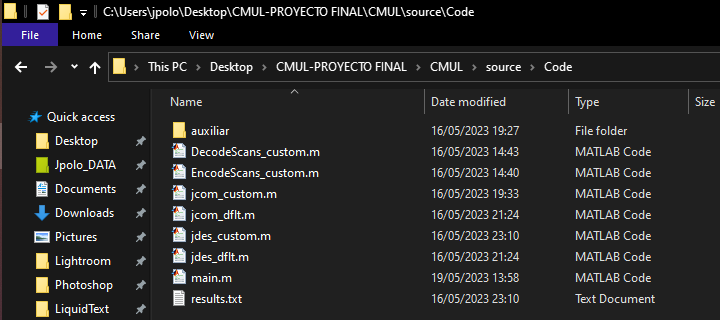
\includegraphics[width=0.30\textwidth]{images/explorer.png}
    \caption[Referencia - explorer]{Imagen original de referencia.}
    
\end{figure}
    
    \vspace{0.5cm}

Imágenes resultantes:
\begin{figure}[H]
    
    \begin{subfigure}{0.30\textwidth}
        \centering
        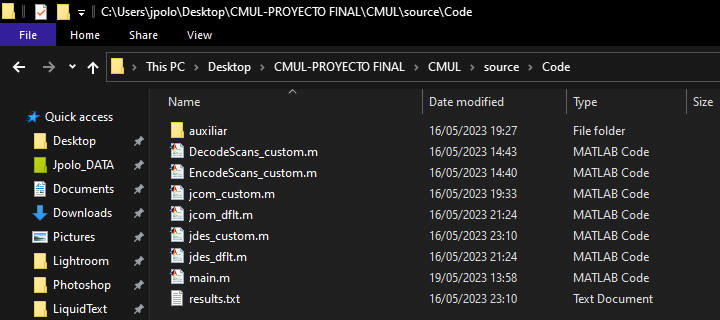
\includegraphics[width=\linewidth]{dflt/explorer_Q50_dec_dflt.png}
        \caption{CaliQ=50.}
        
    \end{subfigure}
    \hfill
    \begin{subfigure}{0.30\textwidth}
        \centering
        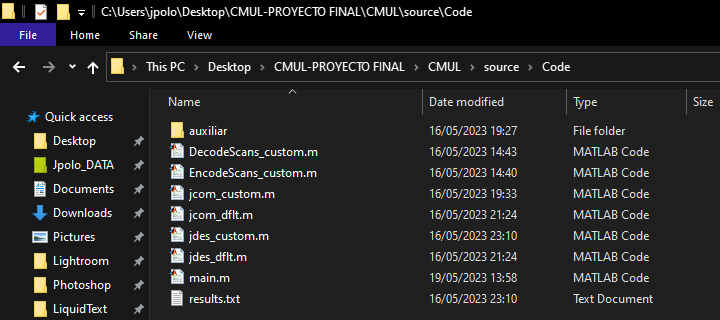
\includegraphics[width=\linewidth]{dflt/explorer_Q100_dec_dflt.png}
        \caption{CaliQ=100.}
        
    \end{subfigure}
    \hfill
    \begin{subfigure}{0.30\textwidth}
        \centering
        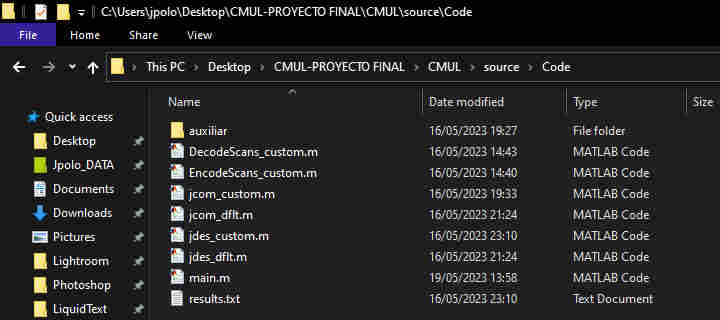
\includegraphics[width=\linewidth]{dflt/explorer_Q250_dec_dflt.png}
        \caption{CaliQ=200.}
        
    \end{subfigure}
    
    \caption[Resultados experimentales - explorer]{Resultados experimentales de la compresión de la imagen \textit{explorer.bmp}.}
    
\end{figure}

Con factor 50 vemos ya cómo el texto se emborrona y aparece una especie de ``halo de píxeles'' alrededor de las letras. El fondo se preserva plano, pero en los elementos como el texto o los iconos se aprecia bastante este efecto que puede dificultar la lectura. Con factor 100 se acentúa este efecto y algunas líneas como la de la barra de direcciones se empiezan a ver dobles. Las palabras podrían ser difícilmente legibles para personas con algún problema de visión. Con factor 200 cuesta distinguir algunas palabras, y elementos gráficos como la chincheta de la barra de acceso rápido son totalmente indistinguibles.\\

Debido a que aquí lo importante es la legibilidad del texto, y vemos que empeora rápidamente, me quedaré con el factor 50.\\

\subsubsection{gradient}
Primero se muestra la imagen original para tener una referencia:
\begin{figure}[H]
    \centering
    
\includegraphics[width=0.25\textwidth]{images/gradient.png}
    \caption[Referencia - gradient]{Imagen original de referencia.}
    
\end{figure}
    
    \vspace{0.5cm}

Imágenes resultantes:
\begin{figure}[H]
    
    \begin{subfigure}{0.25\textwidth}
        \centering
        
\includegraphics[width=\linewidth]{dflt/gradient_Q50_dec_dflt.png}
        \caption{CaliQ=50.}
        
    \end{subfigure}
    \hfill
    \begin{subfigure}{0.25\textwidth}
        \centering
        
\includegraphics[width=\linewidth]{dflt/gradient_Q100_dec_dflt.png}
        \caption{CaliQ=100.}
        
    \end{subfigure}
    \hfill
    \begin{subfigure}{0.25\textwidth}
        \centering
        
\includegraphics[width=\linewidth]{dflt/gradient_Q250_dec_dflt.png}
        \caption{CaliQ=200.}
        
    \end{subfigure}
    
    
    \caption[Resultados experimentales - gradient]{Resultados experimentales de la compresión de la imagen \textit{gradient.bmp}.}
    
\end{figure}

En este caso vemos cómo los resultados coinciden en gran medida con la hipótesis planteada. De la transición gradual y suave de la imagen original se pasa a transiciones de color cada vez más abruptas en regiones escalonadas del mismo color. Es decir, colores parecidos se agrupan en una sola región de un colo único, y el tamaño de esta región crece conforme lo hace Q.\\

Con factor 50 la transición sigue siendo suave y casi imperceptible. Con factor 100 se empieza a ver una textura un poco pixelada y una transición un poco menos suave, pero el efecto se nota poco. Con factor 200 las transiciones son muy abruptas y el resultado no es adecuado visualmente.\\

Elegiré en este caso el factor 100.

\subsubsection{color\_shapes}
Primero se muestra la imagen original para tener una referencia:
\begin{figure}[H]
    \centering
    
\includegraphics[width=0.30\textwidth]{images/cshapes.png}
    \caption[Referencia - color\_shapes]{Imagen original de referencia.}
    
\end{figure}
    
    \vspace{0.5cm}

Imágenes resultantes:
\begin{figure}[H]
    
    \begin{subfigure}{0.30\textwidth}
        \centering
        
\includegraphics[width=\linewidth]{dflt/cshapes_Q50_dec_dflt.png}
        \caption{CaliQ=50.}
        
    \end{subfigure}
    \hfill
    \begin{subfigure}{0.30\textwidth}
        \centering
        \includegraphics[width=\linewidth]{dflt/cshapes_Q100_dec_dflt.png}
        \caption{CaliQ=100.}
        
    \end{subfigure}
    \hfill
    \begin{subfigure}{0.30\textwidth}
        \centering
        \includegraphics[width=\linewidth]{dflt/cshapes_Q250_dec_dflt.png}
        \caption{CaliQ=200.}
        
    \end{subfigure}
    
    \caption[Resultados experimentales - color\_shapes]{Resultados experimentales de la compresión de la imagen \textit{cshapes.bmp}.}
    
\end{figure}

En este ejemplo la clave es ver cómo se comportan los bordes de unión entre regiones de distinto color. El problema principal es que las líneas de unión son diagonales. En las imágenes resultantes vemos cómo los bordes se encuentran difuminados, tanto en la forma como en los colores, que se mezclan y aparecen tonalidades nuevas que no existían en la imagen original. También se pueden apreciar claramente los bloques que conforman la imagen en las líneas diagonales.\\

Sin embargo, al tratarse de una imagen de tamaño pequeño el efecto no es tan notable y considero que con el factor CaliQ=100 todavía es un resultado aceptable. Con CaliQ=200 el efecto es demasiado evidente como para considerarlo satisfactorio.\\


\subsubsection{x-ray}
Primero se muestra la imagen original para tener una referencia:
\begin{figure}[H]
    \centering
    \includegraphics[width=0.30\textwidth]{images/xray.png}
    \caption[Referencia - x-ray]{Imagen original de referencia.}
    
\end{figure}
    
    \vspace{0.5cm}

Imágenes resultantes:
\begin{figure}   [H]
    \begin{subfigure}{0.30\textwidth}
        \centering
        \includegraphics[width=\linewidth]{dflt/xray_Q50_dec_dflt.png}
        \caption{CaliQ=50.}
        
    \end{subfigure}
    \hfill
    \begin{subfigure}{0.30\textwidth}
        \centering
        \includegraphics[width=\linewidth]{dflt/xray_Q100_dec_dflt.png}
        \caption{CaliQ=100.}
        
    \end{subfigure}
    \hfill
    \begin{subfigure}{0.30\textwidth}
        \centering
        \includegraphics[width=\linewidth]{dflt/xray_Q250_dec_dflt.png}
        \caption{CaliQ=200.}
        
    \end{subfigure}
    
    \caption[Resultados experimentales - x-ray]{Resultados experimentales de la compresión de la imagen \textit{xray.bmp}.}
    
\end{figure}

En esta imagen vemos como con factor CaliQ=100 la imagen aparece bastante pixelada, sobre todo el fondo negro. Esto podría  dificultar la interpretación de la radiografía y dar lugar a resultados erróneos (aparecen cosas que no están y viceversa), lo que es totalmente inasumible en este contexto. Por esta razón escogeré el factor más bajo de los propuestos, en este caso CaliQ=50, porque las diferencias que presenta respecto a la original no son tolerables en cualquier otro factor de compresión.\\

Como observación, el texto y la escala de medida se conservan relativamente bien, posiblemente porque las letras no son demasiado pequeñas.\\

Para CaliQ=200 el fondo se encuentra totalmente pixelado y los detalles más finos de los huesos se pierden.


\subsubsection{Conclusiones del estudio cualitativo}

Se ha comprobado cómo los resultados considerados ``adecuados'' varían en las diferentes imágenes, no existe un solo criterio único que sea aplicable a todas.\\

Sin embargo, sí que se pueden extraer algunas conclusiones:\\

El análisis parece indicar que para las imágenes con mayor cantidad de detalles pequeños y diferentes, especialmente elementos que deben ser legibles (explorer, mandrill, x-ray) solo se obtienen buenos resultados si se consideran valores de CaliQ bajos (50 en este caso). Por otro lado, para una imagen que podemos considerar promedio (candados, lennon, lena, gradient) el factor 100 ofrece buenos resultados. Hay que destacar que en casi ningún caso se ha considerado el factor 200 como adecuado, debido a que la pérdida de información con este factor es muy notable.\\

Es importante recordar que este análisis es plenamente subjetivo, y por tanto podría variar según el observador. También hay que destacar que cada imagen se ha analizado en su contexto, dando importancia por ejemplo a la legibilidad del texto si es que lo había o a la importancia de mantener detalles en la radiografía mostrada en \textit{x-ray}.\\

De esta manera, podemos concluir que el valor 100 del factor de calidad CaliQ es el que ofrece mejores resultados visuales subjetivos en la mayoría de las situaciones.\\

\newpage
\subsection{Estudio cuantitativo}
Los resultados obtenidos del estudio cualitativo parecen indicar que un valor adecuado para el factor de calidad podría ser el valor 100.\\

En el estudio cuantitativo, buscaremos responder esta misma pregunta, determinándolo de manera objetiva un valor adecuado para el factor de calidad basándonos en las métricas MSE, RC y SNR mencionadas anteriormente. Comenzaremos discutiendo los resultados obtenidos para cada imagen en particular y luego intentaremos extraer una conclusión global.\\

Es importante recordar que las métricas cuantitativas nos brindan una medida objetiva de la calidad de compresión, pero no siempre reflejan completamente el parecido visual entre la imagen original y la comprimida.\\ 

A continuación, presentaremos los resultados obtenidos para cada imagen individual y analizaremos las métricas MSE, RC y SNR correspondientes con la ayuda de distintas gráficas. Posteriormente, realizaremos una síntesis global de los resultados para determinar un valor adecuado del factor de calidad.\\

Este análisis era subjetivo, ahora vamos a intentar determinar la misma cuestión de forma cuantitativa (y por tanto objetiva), basándonos en las métricas MSE, RC y SNR explicadas anteriormente (\ref{metricasCuant}). \\

Igual que en el análisis cualitativo, discutiremos los resultados en cada imagen particular y luego intentaremos extraer una conclusión global.\\

\subsubsection{candados}
\hspace*{-2.5em}
\begin{minipage}{0.5\textwidth}
        \centering
        \begin{figure}[H]
        \centering
        \includegraphics[scale=0.65]{data/candados_mse.png}
        \caption{log(MSE) vs RC - candados}
        \label{cand-mse}
        \end{figure}
        \end{minipage}\hfill
        \begin{minipage}{0.5\textwidth}
         \begin{figure}[H]
        \centering
        \includegraphics[scale=0.65]{data/candados_snr.png}
        \caption{SNR vs RC - candados}
        \label{cand-snr}
        
        \end{figure}  
\end{minipage}

\vspace{2em}
En la figura \ref{cand-mse} se muestran los valores del MSE en función de los valores de RC. Cada par de valores (MSE,RC) es el que se ha obtenido como resultado de compresión con un valor determinado de calidad CaliQ. Como resulta esperable, cuanto mayor es el valor de CaliQ, mayor es RC (se conservan menos detalles por tanto la tasa de compresión crece, como cabría esperar), por esa razón basta considerar el par de valores descrito, entendiendo que el primer punto se corresponde con lo obtenido para el primer valor de CaliQ, el segundo con el segundo valor y así con todos los demás (esto nos permitirá visualizar los resultados más fácilmente en una gráfica bidimensional, en vez de una de 3 dimensiones).\\ 

Además, para representar el MSE se ha empleado escala logarítmica, debido a que los valores crecen muy rápidamente y dificultaría visualizarlo en escala decimal usual.\\

Una vez realizadas las consideraciones iniciales, vamos a analizar las gráficas obtenidas.\\

Lo primero que podemos observar es que para un mismo factor de calidad, los valores de MSE obtenidos son iguales. Esto resulta esperable si tenemos en cuenta que el MSE cuantifica cuánto se aleja numéricamente una imagen de la imagen original y que cuando se usa un mismo factor de calidad, se descartan los mismos coeficientes de la imagen en el espacio de las frecuencias.\\

Analizaremos por tanto cuál de los dos algoritmos tiene una mayor relación de compresión (RC) para una mismo nivel de pérdida de información. Visualmente, será mejor la gráfica que esté más a la derecha de las dos.\\

En este primer ejemplo, ambos compresores obtienen niveles de compresión prácticamente iguales para cada valor de calidad, con el compresor custom siendo un poco mejor en niveles muy bajos o muy altos de compresión. Observamos cómo a partir del quinto punto (CaliQ=200) el MSE empieza a crecer muy rápido superando el valor 100 (recordemos que estamos en escala logarítmica), por lo que se espera que a partir de este valor el resultado empeore rápidamente.\\

La gráfica \ref{cand-snr} muestra los pares (SNR,CR) para cada valor de calidad CaliQ (el orden de los puntos se corresponde con el valor de CaliQ, como en el caso anterior). Igual que en el caso anterior, para cada valor de calidad, los valores de SNR son los mismos en ambos compresores, de forma que buscaremos cuál es el compresor que obtiene mayor RC para un mismo SNR. Esta gráfica tendrá pendiente negativa, puesto que cuando aumenta la pérdida de información, aumenta el RC pero también aumenta el ruido (y por tanto disminuye SNR).\\

En esta imagen vemos también cómo ambos compresores tienen un desempeño casi idéntico en función del SNR. Se puede observar cómo a partir del quinto punto (CaliQ=200) el valor empieza a decrecer de forma más rápida, empeorando rápidamente a partir de este punto.\\

Observamos cómo parece haber una relación entre el MSE y el SNR en términos de a partir de qué valor de calidad la imagen comienza a empeorar exponencialmente. Con el resto de imágenes comprobaremos si esta relación se mantiene.\\

\subsubsection{lennon}
\hspace*{-2.5em}
\begin{minipage}{0.5\textwidth}
        \centering
        \begin{figure}[H]
    \centering
    \includegraphics[scale=0.65]{data/lennon_mse.png}
    \caption{log(MSE) vs RC - lennon}
    \label{len-mse}
    \end{figure}
    \end{minipage}\hfill
    \begin{minipage}{0.5\textwidth}
        \begin{figure}[H]
    \centering
    \includegraphics[scale=0.65]{data/lennon_snr.png}
    \caption{SNR vs RC - lennon}
    \label{len-snr}
\end{figure}
\end{minipage}
\vspace{2em}

En la primera gráfica vemos que el MSE crece exponencialmente a partir del tercer punto (CaliQ=50), pero se mantiene bastante bajo, superando el valor 100 únicamente en el último punto. Esto nos podría indicar que para esta imagen podríamos aplicar valores de CaliQ elevados (CaliQ=200 o incluso CaliQ=500).\\

Lo mismo ocurre para el SNR, donde la pendiente negativa aumenta tras los primero puntos pero no alcanza valores muy bajos (por encima de 25 en todos los puntos menos el último).\\

En ambos casos la gráfica del compresor custom se encuentra más a la derecha, obteniendo mejores resultados.\\


\subsubsection{lena}
\hspace*{-2.5em}
\begin{minipage}{0.5\textwidth}
        \centering
        \begin{figure}[H]
    \centering
    \includegraphics[scale=0.65]{data/lena_mse.png}
    \caption{log(MSE) vs RC - lena}
    
\end{figure}
\end{minipage}\hfill
    \begin{minipage}{0.5\textwidth}
        \centering
        \begin{figure}[H]
    \centering
    \includegraphics[scale=0.65]{data/lena_snr.png}
    \caption{SNR vs RC - lena}
    
\end{figure}
\end{minipage}
\vspace{2em}

En esta imagen vemos un comportamiento casi idéntico al de la imagen anterior, aunque en ambos compresores se alcanzan valores de ratio de compresión (RC) un poco menores. Esto tiene sentido puesto que ambas imágenes son similares, mostrando un sujeto sobre un fondo con pocos elementos. Probablemente la mayor complejidad de la segunda es lo que explicaría estos resultados un poco peores. Las dos tienen también valores de MSE y SNR muy parecidos.\\

El  MSE empieza a aumentar exponencialmente a partir del cuarto punto. El SNR empieza a disminuir exponencialmente en el mismo punto.
 
\subsubsection{mandrill}
\hspace*{-2.5em}
\begin{minipage}{0.5\textwidth}
        \centering
        \begin{figure}[H]
    \centering
    \includegraphics[scale=0.65]{data/mandrill_mse.png}
    \caption{log(MSE) vs RC - mandrill }
    
\end{figure}
\end{minipage}\hfill
    \begin{minipage}{0.5\textwidth}
        \centering
        \begin{figure}[H]
    \centering
    \includegraphics[scale=0.65]{data/mandrill_snr.png}
    \caption{SNR vs RC - mandrill}
    
\end{figure}
\end{minipage}
\vspace{2em}

Este ejemplo no ofrece resultados muy buenos. Destacar que se necesita alcanzar un valor de CaliQ=100 para alcanzar un ratio de compresión superior al 90\%, pero entonces el MSE se sitúa alrededor de 200 y el SNR por debajo de 20dB. A partir de aquí apenas se consigue mejorar el RC, a costa de aumentar el ruido y el error de la imagen comprimida.\\

Ambos compresores actúan prácticamente igual en este caso.

\subsubsection{noise}
\hspace*{-2.5em}
\begin{minipage}{0.5\textwidth}
        \centering
        \begin{figure}[H]
    \centering
    \includegraphics[scale=0.65]{data/noise_mse.png}
    \caption{log(MSE) vs RC - noise}
    
\end{figure}
\end{minipage}\hfill
    \begin{minipage}{0.5\textwidth}
        \centering
        \begin{figure}[H]
    \centering
    \includegraphics[scale=0.65]{data/noise_snr.png}
    \caption{SNR vs RC - noise}
    
\end{figure}
\end{minipage}
\vspace{2em}


En esta imagen destaca cómo el MSE alcanza valores extremadamente altos. Esto es algo esperable debido a que los valores son aleatorios (no hay correlación), de manera que al eliminar componentes de la transformada inevitablemente hay muchos cambios respecto a la original y aumenta el error. Por eso, si queremos mantener un valor relativamente pequeño del MSE (en torno a 100), conseguimos tasas de compresión muy pequeños (alrededor de 50\%), un resultado muy inferior al resto de ejemplos.\\

Con el SNR ocurre lo mismo, disminuye extremadamente rápido debido a la aparición de ruido con cualquier mínimo cambio que se produzca.\\

Una observación interesante es que para los valores de calidad más altos, se alcanzan cotas de RC cercanas al 100\%. Esto se debe a que la imagen no se puede representar con un número bajo de componentes de la transformada y se desvirtúa hasta que se asemeja cada vez más a una imagen plana.???\\

El compresor custom parece ofrecer mejores resultados con valores de calidad bajos, pero en cuanto aumenta ambos tienen un desempeño prácticamente igual de malo.

\subsubsection{pattern}
\hspace*{-2.5em}
\begin{minipage}{0.5\textwidth}
        \centering
        \begin{figure}[H]
    \centering
    \includegraphics[scale=0.65]{data/pattern_mse.png}
    \caption{log(MSE) vs RC - pattern}
    
\end{figure}
\end{minipage}\hfill
    \begin{minipage}{0.5\textwidth}
        \centering
        \begin{figure}[H]
    \centering
    \includegraphics[scale=0.65]{data/pattern_snr.png}
    \caption{SNR vs RC - pattern}
    
\end{figure}
\end{minipage}
\vspace{2em}

Este caso resulta curioso porque a priori la regularidad del patrón debería ofrecer buenos resultados en la compresión. Sin embargo, vemos que aumenta el MSE rápidamente hasta alcanzar valores elevados (MSE=1000 con CaliQ=200). Con el SNR sucede lo mismo, a partir del cuarto punto los valores son muy bajos como para poder considerarlos satisfactorios.\\

Este es un caso en el que la diferencia visual subjetiva no es muy alta pero el MSE sí.\\

El compresor custom parece funcionar un poco mejor en este caso.\\


\subsubsection{color\_bars}
\hspace*{-2.5em}
\begin{minipage}{0.5\textwidth}
        \centering
        \begin{figure}[H]
    \centering
    \includegraphics[scale=0.65]{data/color_bars_mse.png}
    \caption{log(MSE) vs RC - color\_bars}
    
\end{figure}
\end{minipage}\hfill
    \begin{minipage}{0.5\textwidth}
        \centering
        \begin{figure}[H]
    \centering
    \includegraphics[scale=0.65]{data/color_bars_snr.png}
    \caption{SNR vs RC - color\_bars}
    
\end{figure}
\end{minipage}
\vspace{2em}

Este es el caso más interesante. La imagen se había considerado con la intención de ofrecer un caso mucho más favorable para el compresor custom que para el compresor default debido a que existen muy pocos tipos de píxeles que aparecen muchas veces al ser todo líneas verticales de unos pocos colores (y el compresor custom asigna códigos más bajos en función de la frecuencia de aparición).\\

Aunque ambos compresores ofrecen unos resultados excelentes (errores muy bajos, SNR alto y ratios de compresión de casi el 100\%), el compresor custom es claramente superior, con resultados de compresión para CaliQ=5 mejores que el compresor default para CaliQ=1000.\\

\subsubsection{explorer}
\hspace*{-2.5em}
\begin{minipage}{0.5\textwidth}
        \centering
        \begin{figure}[H]
    \centering
    \includegraphics[scale=0.65]{data/explorer_mse.png}
    \caption{log(MSE) vs RC - explorer}
    
\end{figure}
\end{minipage}\hfill
    \begin{minipage}{0.5\textwidth}
        \centering
        \begin{figure}[H]
    \centering
    \includegraphics[scale=0.65]{data/explorer_snr.png}
    \caption{SNR vs RC - explorer}
    
\end{figure}
\end{minipage}
\vspace{2em}

En esta imagen se obtienen resultados buenos de compresión para factores de calidad bajos (alrededor de 90\% para CaliQ=25), pero luego (a partir de CaliQ=50) empeora rápidamente, aumentando el MSE por encima de 100 y disminuyendo el SNR debajo de 20dB.\\

El compresor custom parece que funciona un poco mejor que el default, pero no podemos decir que esta diferencia sea muy significativa cuando crece el factor CaliQ.\\


\subsubsection{gradient}
\hspace*{-2.5em}
\begin{minipage}{0.5\textwidth}
        \centering
        \begin{figure}[H]
    \centering
    \includegraphics[scale=0.65]{data/gradient_mse.png}
    \caption{log(MSE) vs RC - gradient}
    
\end{figure}
\end{minipage}\hfill
    \begin{minipage}{0.5\textwidth}
        \centering
        \begin{figure}[H]
    \centering
    \includegraphics[scale=0.65]{data/gradient_snr.png}
    \caption{SNR vs RC - gradient}
    
\end{figure}
\end{minipage}
\vspace{2em}

Estos resultados son curiosos debido a que valores pequeños de CaliQ ofrecen ratios de compresión bastante elevados (más del 95\%) con buenos valores de MSE y SNR, pero a partir del 4º punto (CaliQ=100), el MSE se dispara exponencialmente y el SNR disminuye de la misma forma. Esto nos indica que a partir del valor 100, no se gana apenas en RC y los resultados empeoran considerablemente.\\

Una vez más el compresor custom tiene un desempeño mejor que el compresor default.


\subsubsection{color\_shapes}
\hspace*{-2.5em}
\begin{minipage}{0.5\textwidth}
        \centering
        \begin{figure}[H]
    \centering
    \includegraphics[scale=0.65]{data/cshapes_mse.png}
    \caption{log(MSE) vs RC - color\_shapes}
    
\end{figure}
\end{minipage}\hfill
    \begin{minipage}{0.5\textwidth}
        \centering
        \begin{figure}[H]
    \centering
    \includegraphics[scale=0.65]{data/cshapes_snr.png}
    \caption{SNR vs RC - color\_shapes}
    
\end{figure}
\end{minipage}
\vspace{2em}

En este caso se alcanzan ratios de compresión elevados (más del 95\% a partir de CaliQ=25), lo que tiene sentido teniendo en cuenta que hay grandes áreas del mismo color y no hay detalles excepto en las fronteras entre colores. El MSE aumenta de forma lineal hasta CaliQ=100, donde aumenta la pendiente. Con el SNR sucede de manera análoga decreciente. Esto nos indica que el valor 100 puede ser un buen valor para tomar, a partir de ese punto la imagen empeora y no hay tanta ganancia en RC.

\subsubsection{x-ray}
\hspace*{-2.5em}
\begin{minipage}{0.5\textwidth}
        \centering
        \begin{figure}[H]
    \centering
    \includegraphics[scale=0.65]{data/xray_mse.png}
    \caption{log(MSE) vs RC - x-ray}
    
\end{figure}
\end{minipage}\hfill
    \begin{minipage}{0.5\textwidth}
        \centering
        \begin{figure}[H]
    \centering
    \includegraphics[scale=0.65]{data/xray_snr.png}
    \caption{SNR vs RC - x-ray}
    
\end{figure}
\end{minipage}
\vspace{2em}

En este ejemplo se consiguen (CaliQ=100) tasas de compresión de alrededor del 98\% con un MSE bastante bajo de alrededor de 50 y un SNR superior a 20bB (valores mejores que en muchos de los ejemplos anteriores). A partir de este punto la calidad de la imagen resultante empeora sin mejorar la RC significativamente.\\

El compresor custom es ligeramente mejor al default en este ejemplo.

\subsubsection{Conclusiones del estudio cuantitativo}
En los ejemplos anteriores se ha analizado la evolución de las diferentes métricas (RC,MSE,SNR) en función del valor del factor de calidad CaliQ escogido. Se ha visto en qué ejemplos se conseguían mayores ratios de compresión con un MSE menor y un SNR mayor, en cuáles se disparaba el error y en cuáles se mantenía en niveles más bajos (respectivamente con el SNR).\\

De aquí podemos extraer varias conclusiones:\\

Para empezar, los datos obtenidos señalan un mejor desempeño del compresor custom en más de la mitad de los ejemplos probados (concretamente en 6 de los 11 ejemplos). En aquellos ejemplos en los que este compresor no era claramente superior, ambos obtenían resultados prácticamente idénticos. Esto parece indicar que el compresor custom obtiene mejores resultados en general (aunque habría que realizar una prueba más exhaustiva con una batería de imágenes mucho mayor para poder obtener conclusiones más firmes).\\

También se ha determinado que en 9 de las 11 imágenes analizadas se alcanza claramente un punto a partir del cual el MSE se dispara y el SNR disminuye rápidamente. Esto indicaría que a partir de ese punto la pérdida de información en la imagen comprimida aumentaría exponencialmente, sin proporcionar aumentos notables en el ratio de compresión (RC). Para intentar establecer un criterio objetivo basado únicamente en estos datos, podríamos considerar que el valor adecuado del factor de compresión CaliQ para emplear con los compresores será precisamente este. De esta manera se intenta maximizar la compresión sin que la imagen pierda excesiva calidad.\\

En 5 de las 9 ocasiones en las que el este fenómeno de crecimiento se ha percibido se ha determinado que el punto óptimo es el cuarto, correspondiente al factor de calidad CaliQ=100. Los otros dos valores que más se repiten son CaliQ=50 (2/9) y CaliQ=200 (2/9). Este resultado coincide con el que se obtuvo en el análisis cualitativo, lo que refuerza la fiabilidad de estas conclusiones.\\

De esta manera, por los datos obtenidos podríamos concluir que la configuración óptima del compresor para un caso general sería utilizar el \textbf{compresor Custom con factor de calidad CaliQ=100}. \\

Como observaciones finales, los ejemplos en los que los dos compresores obtienen resultados prácticamente idénticos son precisamente las imágenes en las que más detalles diferentes había (candados, mandrill, noise) y por tanto menos correlación de la que poder sacar partido, sobre todo el compresor custom. Son también las imágenes en las que peores resultados se obtienen. Es decir, el compresor custom funciona mejor en los casos promedio y en los casos extremos los dos funcionan igual (de mal).\\

\subsubsection{Extra: Análisis de SSIM}
Al realizar el análisis cuantitativo solo se está teniendo en cuenta la diferencia ``numérica'' entre la imagen comprimida y la original, mediante un criterio únicamente matemático bajo la premisa de que las diferencias ``reales'' que existen entre las imágenes se traducen en diferencias percibidas por el observador. Esto es así en la mayoría de los casos, pero en otros (por ejemplo, en la imagen \textit{pattern} analizada anteriormente), no tiene por qué ser así.\\

Si investigamos sobre el tema, encontramos una métrica utilizada con frecuencia en el estudio de algoritmos de compresión que permite aunar hasta cierto punto el análisis cuantitativo con la percepción visual de la imagen. Se trata del SSIM \cite{Imatest-SSIM}.\\

A diferencia del MSE y la SNR, el SSIM tiene en cuenta la estructura y la similitud perceptual de las imágenes. Evalúa la similitud de luminancia, el contraste y la estructura y proporciona una evaluación más centrada en cómo los humanos perciben y procesan visualmente las imágenes ya que considera la preservación de detalles, bordes y texturas en lugar de medir solo las diferencias de píxeles (MSE) o la relación señal a ruido (SNR). No deja de ser un análisis numérico pero los datos evaluados parecen estar más relacionados con el resultado final de percepción de un observador humano.\\

Por esta razón, decidimos ampliar el código de la práctica para calcular la métrica SSIM, para ver si nos aporta alguna información extra que sea relevante.\\

Para ello se ha utilizado la función \textit{ssim(A,ref)} de la librería de \textit{Matlab}  \cite{mathworks-ssim}, puesto que la implementación manual sería compleja y escaparía del ámbito de este trabajo. Esta función calcula el valor de la métrica SSIM entre una imagen (en nuestro caso la imagen comprimida) y la imagen de referencia (en nuestro caso la original).\\

Calculamos este valor para cada una de las combinaciones de compresor-factor de calidad y para todas las imágenes y obtenemos los siguientes resultados:\\





\newpage
\section{Conclusión}

?????????????????????????\\
En resumen, la compresión de imágenes se ha convertido en un campo de investigación crucial para hacer frente a la creciente cantidad de datos visuales generados y consumidos en la era digital. El compresor Huffman y la transformada discreta del coseno han demostrado ser herramientas esenciales en este contexto, al permitir una compresión eficiente y preservar la información visual clave. Con la aplicación de estas técnicas y su continua mejora, se busca garantizar una transmisión y almacenamiento óptimos de imágenes, impulsando así el intercambio de conocimientos, la comunicación visual y el desarrollo de tecnologías futuras.\\
?????????????????????????



\newpage
\nocite{*}
\printbibliography


\end{document}